\documentclass[12pt, a4paper, oneside]{report}
%
%
\usepackage{counttexruns}
%%%%%%%%% Preamble file %%%%%%%%%%%%%%
%%%%%%% PACKAGES LOADING %%%%%%%%%%%
%
%
\usepackage[bottom]{footmisc} %keep footnote sticked at the end of the page
%
%
\usepackage{url} %Tratamiento de las urls
\def\UrlBreaks{\do\.\do\@\do\\\do\/\do\!\do\_\do\|\do\;\do\>\do\]%
 \do\)\do\,\do\?\do\'\do+\do\=\do\#\do\&\do\a\do\b\do\c\do\d\do\e%
 \do\f\do\g\do\h\do\i\do\j\do\k\do\l\do\m\do\n\do\o\do\p\do\q\do\r%
 \do\s\do\t\do\u\do\v\do\w\do\x\do\y\do\z\do\A\do\B\do\C\do\D\do\E%
 \do\F\do\G\do\H\do\I\do\J\do\K\do\L\do\M\do\N\do\O\do\P\do\Q\do\R%
 \do\S\do\T\do\U\do\V\do\W\do\X\do\Y\do\Z\do\1\do\2\do\3\do\4\do\5%
 \do\6\do\7\do\8\do\9\do\0}%
%%%%%%%%%%%%%%%%%%%%%%%%%%%%%%%%%%%%
%
%
%%%%%%%% Page Geometry %%%%%%%%%%%%%
\usepackage[top=6cm,bottom=3cm,headheight=4cm, headsep=1cm, footskip=2cm]{geometry}
\usepackage{pdflscape}
%%%%%%%%%%%%%%%%%%%%%%%%%%%%%%%%%%%%
%
%
%%%%%%%%%% Dummy content %%%%%%%%%%%
\usepackage{lipsum}
%%%%%%%%%%%%%%%%%%%%%%%%%%%%%%%%%%%%
%
%
%%%%%%%%% Font & Language %%%%%%%%%%
% XeLaTeX compiler
\usepackage{xltxtra,fontspec,xunicode}
\setsansfont{Verdana}
\usepackage{microtype}
%%%%%%%%%%%%%%%%%%%%%%%%%%%%%%%%%%%%
%
%
%% Enlarge the badboxes tolerances %
\hfuzz=20pt
\vfuzz=20pt
\hbadness=2000
\vbadness=\maxdimen
\emergencystretch 3em%
%
%
%%%%%%%%%%%% Language %%%%%%%%%%%%%
\usepackage[spanish]{babel}
%%%%%%%%%%%%%%%%%%%%%%%%%%%%%%%%%%%%%%
%
%
%%%%%%%%% Floating %%%%%%%%%%%%%%%%%%%
\usepackage{floatrow}
\usepackage{fixmath}
%%%%%%%%%%%%%%%%%%%%%%%%%%%%%%%%%%%%%%
%
%
%%%%%%% Colors & Graphics %%%%%%%%%%%%
\usepackage{amssymb}
\usepackage{soul}
\usepackage{subcaption}
\usepackage[space]{grffile}
\usepackage{tikz}
\usepackage[tikz]{bclogo}
\usetikzlibrary{positioning, arrows, intersections, calc, through, backgrounds, patterns,shapes.geometric}
\usepackage{pgfplots,pgfplotstable}
\usepgfplotslibrary{polar}
\usepackage[american,siunitx]{circuitikz}
\usetikzlibrary{arrows}
\usepackage{lettrine}
\usepackage{amsfonts}
\usepackage{placeins}
\usepackage{longtable}
\usepackage{pgfkeys}
\usepackage{mathtools}
\usetikzlibrary{calc,fadings,decorations.pathreplacing}
%%%%%%%%%%%%%%%%%%%%%%%%%%%%%%%%%%%%%%
%
%
%%%%%%%%%%%%%%% ToC %%%%%%%%%%%%%%%%%%
\setcounter{tocdepth}{2} % Table Of Content depth
%%%%%%%%%%%%%%%%%%%%%%%%%%%%%%%%%%%%%%
%
%
%%%%%%%%%%%%%%% Math %%%%%%%%%%%%%%%%%
\usepackage{amsmath}
\usepackage{amsfonts}
\usepackage{amssymb}
\usepackage{cancel}
\usepackage{units}
\newenvironment{sisalign}{\begin{equation}\left\{\begin{aligned}{}}{\end{aligned}\right.\end{equation}}
\makeatletter
\renewcommand*\env@matrix[1][*\c@MaxMatrixCols c]{%
  \hskip -\arraycolsep
  \let\@ifnextchar\new@ifnextchar
  \array{#1}}
\makeatother %in order to draw vertical lines in bmatrix environment
%%%%%%%%%%%%%%%%%%%%%%%%%%%%%%%%%%%%%%
%
%
%%%%%%%%% Tables Utilities %%%%%%%%%%%
\usepackage{array}
\usepackage{multirow}
\usepackage{booktabs}
\usepackage{longtable}
\usepackage{tabularx}
\usepackage{multicol}
\usepackage{rotating}
\usepackage{tabularx}
\setlength{\tabcolsep}{10pt}
\newcolumntype{L}[1]{>{\raggedright\let\newline\\\arraybackslash\hspace{0pt}}m{#1}}
\newcolumntype{C}[1]{>{\centering\let\newline\\\arraybackslash\hspace{0pt}}m{#1}}
\newcolumntype{R}[1]{>{\raggedleft\let\newline\\\arraybackslash\hspace{0pt}}m{#1}}
%%%%%%%%%%%%%%%%%%%%%%%%%%%%%%%%%%%%%%
%
%
%%%%%%%% Headers Utilities %%%%%%%%%%%
\usepackage{fancyhdr}
\usepackage{lastpage}
%%%%%%%%%%%%%%%%%%%%%%%%%%%%%%%%%%%%%%
%
%
%%%%%%%%%%%%% Codes %%%%%%%%%%%%%%%%%%
\usepackage{listings}  % Source code
\usepackage{moreverb}  % For including source code with tabs
%%%%%%%%%%%%%%%%%%%%%%%%%%%%%%%%%%%%%%
%
%
%%%%%%%%%%%%%% Various %%%%%%%%%%%%%%%
\usepackage{counttexruns}
\usepackage{textcomp}
\usepackage{parskip}
\usepackage{ifthen}
\usepackage{nameref}
\usepackage{enumerate}
\usepackage{placeins}   % Avoid floating frames to be too floating...
\usepackage{eurosym}	% Include euro symbol
\renewcommand{\labelitemi}{$\vartriangleright$}
\renewcommand{\labelitemii}{$\circ$}
%%%%%%%%%%%%%%%%%%%%%%%%%%%%%%%%%%%%%%
%
%
%%%%%%%%%%%% HyperLinks %%%%%%%%%%%%%%
\usepackage[hidelinks]{hyperref}
\hypersetup{%
pdfpagemode={UseOutlines},
bookmarksopen,
pdfstartview={FitH},
plainpages=false
%colorlinks,
%linkcolor={gray},
%citecolor={gray},
%urlcolor={blue}
}
%%%%%%%%%%%%%%%%%%%%%%%%%%%%%%%%%%%%%%
%
%
%%%%%%%%%%%% Bibliography %%%%%%%%%%%%
\usepackage{apacite}
%%%%%%%%%%%%%%%%%%%%%%%%%%%%%%%%%%%%%%
%
%
%%%%%%%%%%%%%%% EPS %%%%%%%%%%%%%%%%%%
\usepackage{epstopdf}
%%%%%%%%%%%%%%%%%%%%%%%%%%%%%%%%%%%%%%
%
%
%%%%%%%% Equations spaces %%%%%%%%%%%%
\let\originalequation\equation
\let\endoriginalequation\endequation
\renewenvironment{equation}
{%
  \originalequation
  \addtolength\abovedisplayshortskip{15pt}
  \addtolength\abovedisplayskip{15pt}
  \addtolength\belowdisplayshortskip{15pt}
  \addtolength\belowdisplayskip{15pt}}
{\endoriginalequation \ignorespacesafterend}
%
\let\originaldisplaymath\displaymath
\let\endoriginaldisplaymath\enddisplaymath
\renewenvironment{displaymath}
{%
  \originaldisplaymath
  \addtolength\abovedisplayshortskip{15pt}
  \addtolength\abovedisplayskip{15pt}
  \addtolength\belowdisplayshortskip{15pt}
  \addtolength\belowdisplayskip{15pt}}
{\endoriginaldisplaymath \ignorespacesafterend}
%%%%%%%%%%%%%%%%%%%%%%%%%%%%%%%%%%%%%%
%
%
%%%%%% Roman Numerals in Text %%%%%%%%
\makeatletter
\newcommand*{\rom}[1]{\expandafter\@slowromancap\romannumeral #1@}
\makeatother
%%%%%%%%%%%%%%%%%%%%%%%%%%%%%%%%%%%%%%
%
%
%% Change Chapter & Section Format %%%
\usepackage{titlesec}
%
\titleformat{\chapter}[display]
{\normalfont\rmfamily\Large\centering}
{\chaptertitlename\ \thechapter}{0pt}{\Huge}
%
\titleformat{\section}
{\normalfont\rmfamily\bfseries}
{\thesection}{1em}{}
%
\titleformat{\subsection}
{\normalfont\rmfamily \slshape}
{\thesubsection}{12pt}{}[]
%
%%%%%%%%%%%%%%%%%%%%%%%%%%%%%%%%%%%%%%
%
%
%%%%% Date format (XX/XX/XXXX) %%%%%%%
\usepackage{datetime}
\newdateformat{dateFMT}
{%
	\twodigit{\THEDAY}/\twodigit{\THEMONTH}/\THEYEAR
}
\newdateformat{monthyeardate}
{%
	\monthname[\THEMONTH] de \THEYEAR
}
%%%%%%%%%%%%%%%%%%%%%%%%%%%%%%%%%%%%%%
%
%
%%%%%% Headers Definition %%%%%%%%%%%%
\headheight=70pt
\fancyheadoffset[L,R]{1cm}
\fancyfootoffset[L,R]{1cm}
\pagestyle{fancy}
\rhead{}
\lhead{}
\chead{\fancyplain{}{%
\renewcommand{\arraystretch}{1.2}
\resizebox{\textwidth}{!}{
\begin{tabular}{l c l}
\toprule
\multirow{3}[2]{*}{
\includegraphics[width=25mm]{Logo/uemc_logo.pdf}} & \multirow{3}{*}{\begin{minipage}{7cm}\begin{center} \textbf{\project} \end{center} \ifthenelse{\equal{\projectshort}{}}{\project}{} \end{minipage}} & Date:\printDate \\
&       & Ed.: \\
&       & Pag.:\thepage\ of \pageref{LastPage}\\ \bottomrule
\end{tabular}}}
}
\renewcommand{\headrulewidth}{0pt}
%%%%%%%%%%%%%%%%%%%%%%%%%%%%%%%%%%%%%%
%
%
%%%%%%%%%%%% COVER PAGE %%%%%%%%%%%%%%
\newlength{\drop}
\newcommand*{\coverPage}
{
	\begingroup%
	\drop=0.1\textheight
	%\vspace*{\drop}
	\vspace*{-2cm}
	\centering
	{
		{\sffamily\fontsize{18}{30}\selectfont%
		\textbf{UNIVERSIDAD EUROPEA\\ \vspace*{10pt}MIGUEL DE CERVANTES}}
		\par
		\vspace*{30pt}
		{\sffamily\fontsize{16}{28}\selectfont%
		\textbf{ESCUELA POLITÉCNICA SUPERIOR}}
		\par
		\vspace*{20pt}
		{\sffamily\fontsize{14}{28}\selectfont%
		\textbf{TITULACIÓN:\\ \vspace*{1pt}MÁSTER UNIVERSITARIO EN GESTIÓN Y ANÁLISIS DE GRANDES VOLÚMENES DE DATOS: BIG DATA}}
		\par
		{
\includegraphics[width=160pt]{Logo/escudo_UEMC.png}}
		\par
		\vspace*{-5pt}
		{\sffamily\fontsize{16}{28}\selectfont%
		\textbf{TRABAJO FIN DE MÁSTER}}
		\par
		\vspace*{30pt}
		{\sffamily\fontsize{22}{34}\selectfont%
		\textbf{\project}}
		\par
		\vspace*{30pt}
		{\sffamily\fontsize{14}{28}\selectfont%
		\textbf{AUTOR}}
		\par
		\vspace*{10pt}
		{\sffamily\fontsize{16}{28}\selectfont%
		\textbf{\authorname}}
		\par
		\vspace*{10pt}
		{\sffamily\fontsize{14}{28}\selectfont%
		\textbf{TUTOR}}
		\par
		\vspace*{10pt}
		{\sffamily\fontsize{16}{28}\selectfont%
		\textbf{\tutoredby}}
		\par
		\vspace*{10pt}
		{\sffamily\fontsize{14}{28}\selectfont%
		\textbf{VALLADOLID, \monthyeardate\today}}
		\par
	}\par
	\endgroup
}
%%%%%%%%%%%%%%%%%%%%%%%%%%%%%%%%%%%%%%
%% ARROW
\newcommand{\arrowTikz}[1]
{
	\begin{tikzpicture}[rotate=#1]
		\coordinate (initPoint)   at (0,0);
		\coordinate (endingPoint) at (0.5,0);
		\draw [line width=1pt,-{Stealth[length=3pt,width=4pt,inset=0.3pt]}](initPoint)--(endingPoint);
	\end{tikzpicture}
}

%% SECTION AND SUBSECTIONS REFERENCE
\newcommand{\refsec}[1]{section~\ref{#1}}
\newcommand{\refsubsec}[1]{subsecsection~\ref{#1}}

%% SUPER & SUB SCRIPT
\newcommand{\superscript}[1]{\ensuremath{^{\textrm{#1}}}}
\newcommand{\subscript}[1]{\ensuremath{_{\textrm{#1}}}}
%% BOLD ITEM
\newcommand\litem[1]{\item{\bfseries #1\enspace} \\}
%% WRITE A VECTOR IN BOLD
\newcommand{\bvec}[1]{\vec{\mathbf{#1}}}
%% PARTIAL DERIVATIVE
\newcommand{\pdv}[2]{\frac{\partial #1}{\partial #2}}
%% BIGO
\DeclareMathAlphabet{\mathpzc}{OT1}{pzc}{m}{it}
\newcommand{\bigO}[1]{$\mathpzc{O}(#1)$}
%% FOR TABLES
\newfloatcommand{capbtabbox}{table}[][\FBwidth]
%% EARTH SPHERE DRAWING
\newcommand\pgfmathsinandcos[3]{%
	\pgfmathsetmacro#1{sin(#3)}%
	\pgfmathsetmacro#2{cos(#3)}%
}
\newcommand\LongitudePlane[3][current plane]{%
	\pgfmathsinandcos\sinEl\cosEl{#2} % elevation
	\pgfmathsinandcos\sint\cost{#3} % azimuth
	\tikzset{#1/.style={cm={\cost,\sint*\sinEl,0,\cosEl,(0,0)}}}
}
\newcommand\LatitudePlane[3][current plane]{%
	\pgfmathsinandcos\sinEl\cosEl{#2} % elevation
	\pgfmathsinandcos\sint\cost{#3} % latitude
	\pgfmathsetmacro\yshift{\cosEl*\sint}
	\tikzset{#1/.style={cm={\cost,0,0,\cost*\sinEl,(0,\yshift)}}} %
}
\newcommand\DrawLongitudeCircle[2][1]{
	\LongitudePlane{\angEl}{#2}
	\tikzset{current plane/.prefix style={scale=#1}}
	% angle of "visibility"
	\pgfmathsetmacro\angVis{atan(sin(#2)*cos(\angEl)/sin(\angEl))} %
	\draw[current plane] (\angVis:1) arc (\angVis:\angVis+180:1);
	\draw[current plane,dashed] (\angVis-180:1) arc (\angVis-180:\angVis:1);
}
\newcommand\DrawLongitudeCircleRed[2][1]{
	\LongitudePlane{\angEl}{#2}
	\tikzset{current plane/.prefix style={scale=#1}}
	% angle of "visibility"
	\pgfmathsetmacro\angVis{atan(sin(#2)*cos(\angEl)/sin(\angEl))} %
	\draw[current plane, color = red] (\angVis:1) arc (\angVis:\angVis+180:1);
	\draw[current plane,dashed, color = red] (\angVis-180:1) arc (\angVis-180:\angVis:1);
}
\newcommand\DrawLatitudeCircle[2][2]{
	\LatitudePlane{\angEl}{#2}
	\tikzset{current plane/.prefix style={scale=#1}}
	\pgfmathsetmacro\sinVis{sin(#2)/cos(#2)*sin(\angEl)/cos(\angEl)}
	% angle of "visibility"
	\pgfmathsetmacro\angVis{asin(min(1,max(\sinVis,-1)))}
	\draw[current plane] (\angVis:1) arc (\angVis:-\angVis-180:1);
	\draw[current plane,dashed] (180-\angVis:1) arc (180-\angVis:\angVis:1);
}
\newcommand\DrawLatitudeCircleRed[2][2]{
	\LatitudePlane{\angEl}{#2}
	\tikzset{current plane/.prefix style={scale=#1}}
	\pgfmathsetmacro\sinVis{sin(#2)/cos(#2)*sin(\angEl)/cos(\angEl)}
	% angle of "visibility"
	\pgfmathsetmacro\angVis{asin(min(1,max(\sinVis,-1)))}
	\draw[current plane,red] (\angVis:1) arc (\angVis:-\angVis-180:1);
	\draw[current plane,dashed,red] (180-\angVis:1) arc (180-\angVis:\angVis:1);
}

%% CAPTION FOR EQUATION SET
\newcounter{equationset}
\newcommand{\equationset}[1]{% \equationset{<caption>}
	\refstepcounter{equationset}% Step counter
	\noindent\makebox[\linewidth]{Ecuaci\'on~\theequationset: #1}}% Print caption
%%%%%%%%%%%%%%%%%%%%%%%%%%%%%%%%%%%%%%
%
%

%%%%%%%%%%%%%% Glossary %%%%%%%%%%%%%%
\usepackage{glossaries}
\makeglossaries
% Definitions and acronyms entries

% \newacronym{uav}{UAV}{Unmanned Aerial Vehicle}
% Reference singular: \gls{uav}   --> UAV
% Reference plural:   \glspl{uav} --> UAVs

% The following definitions will go in the main glossary

% Basics
\newacronym{TFM}{TFM}{Trabajo de Fin de Máster}
\newacronym{UEMC}{UEMC}{Universidad Europea Miguel de Cervantes}
\newacronym{TTF}{TTF}{TrueType Font}
\newacronym{OTF}{OTF}{OpenType Font}
\newacronym{WWW}{WWW}{World Wide Web}
\newacronym{HTTP}{HTTP}{HyperText Transfer Protocol}
\newglossaryentry{framework}{name={Framework},description={Un framework, entorno de trabajo​ o marco de trabajo​ es un conjunto estandarizado de conceptos, prácticas y criterios para enfocar un tipo de problemática particular que sirve como referencia, para enfrentar y resolver nuevos problemas de índole similar.}}
\newglossaryentry{scraper}{name={Web scraping},description={Es una técnica utilizada mediante programas de software para extraer información de sitios web.1​ Usualmente, estos programas simulan la navegación de un humano en la \gls{WWW} ya sea utilizando el protocolo \gls{HTTP} manualmente, o incrustando un navegador en una aplicación.}}
\newacronym{API}{API}{Application Programming Interface}
\newacronym{HTML}{HTML}{HyperText Markup Language}
\newacronym{JSON}{JSON}{JavaScript Object Notation}
\newacronym{URL}{URL}{Uniform Resource Locator}
\newglossaryentry{GET}{name={GET},description={Es un método de petición del protocolo \gls{HTTP} que se utiliza para solicitar datos a través unos filtros definidos en la \gls{URL} con la que se hace la petición.}}
\newglossaryentry{HDF5}{name={HDF5},description={\gls{HDF} versión 5. Es un formato binario organizado utilizado para almacenar y acceder a grandes volúmenes de datos de manera indexada. Está estructurado de manera similar a una carpeta, soporta links virtuales para referenciar datasets, valores de relleno por defecto y metadatos, entre otras capacidades.}}
\newacronym{HDF}{HDF}{Hierarchical Data Format}
\newacronym{RAM}{RAM}{Random Access Memory}
\newacronym{HDD}{HDD}{Hard Disk Drive}
\newacronym{AMD}{AMD}{Advanced Micro Devices}
\newacronym{ROC}{ROC}{Radeon Open Compute}
\newglossaryentry{ROCm}{name={ROCm},description={\gls{ROC}m es un \gls{framework} de código abierto para desarrolladores utilizado para realizar cálculos computacionales en gráficas \gls{AMD} Radeon}}

\newacronym{ADC}{ADC}{Analogical to Digital Converter}
\newacronym{DSP}{DSP}{Digital Signal Procesing}
\newacronym{ASCII}{ASCII}{American Standard Code for Information Interchange}
\newacronym{FPGA}{FPGA}{Field Programmable Gate Array}
\newacronym{AWS}{AWS}{Amazon Web Services}

%% MACHINE LEARNING
\newglossaryentry{dataset}{name={Dataset},description={Conjunto de datos, normalmente estructurados.}}
\newacronym{ML}{ML}{Machine Learning}
\newacronym{LSTM}{LSTM}{Long Short-Term Memory}
\newacronym{GRU}{GRU}{Gated Recurrent Unit}

%% OTHER
\newacronym{GPS}{GPS}{Global Positioning System}

%% DSP
\newacronym{FFT}{FFT}{Fast Fourier Transform}
\newacronym{SNR}{SNR}{Signal to Noise Ratio}
\newacronym{STFT}{STFT}{Short-Time Fourier Transform} % Archivo con las entradas del glosario
%%%%%%%%%%%%%%%%%%%%%%%%%%%%%%%%%%%%%%
%
%
%%%%%%%%%%% DOCUMENT DATA %%%%%%%%%%%%
\newcommand{\project}{Title of the project}
\newcommand{\projectshort}{Short Title}
\newcommand{\authorname}{Ignazio F.Finazzi}
\newcommand{\tutoredby}{Tutor Name and Surname}
\newcommand{\company}{Universidad Europea Miguel de Cervantes}
\newcommand{\doctype}{Draft} %or draft
\newcommand{\revision}{\thecounttexruns}
\newcommand{\printDate}{\dateFMT\today}
%%%%%%%%%%%%%%%%%%%%%%%%%%%%%%%%%%%%%%
%
%
%%%%%%%%%%% PDF METADATA %%%%%%%%%%%%%
\hypersetup{pdftitle={\project},
	pdfauthor={Ignazio F.Finazzi},
	pdfsubject={\project},
	pdfkeywords={\company}
}
%%%%%%%%%%%%%%%%%%%%%%%%%%%%%%%%%%%%%%
%
%
%%%%%%%%% DRAFt TWATERMARK %%%%%%%%%%%
\ifthenelse{\equal{\doctype}{Draft} \or \equal{\doctype}{draft}}
{
	\usepackage[angle=60,
				color=black!40,
				scale=5]{background}}{}
	\backgroundsetup{contents={DRAFT \printDate}}
%%%%%%%%%%%%%%%%%%%%%%%%%%%%%%%%%%%%%%
%
%
%%%%%%%%%%% LISTINGS SETS %%%%%%%%%%%%
\usepackage{color}
%% HTML
\definecolor{editorLightGray}{cmyk}{0.05, 0.05, 0.05, 0.1}
\definecolor{editorGray}{cmyk}{0.6, 0.55, 0.55, 0.2}
\definecolor{editorPurple}{cmyk}{0.5, 1, 0, 0}
\definecolor{editorWhite}{cmyk}{0, 0, 0, 0}
\definecolor{editorBlack}{cmyk}{1, 1, 1, 1}
\definecolor{editorOrange}{cmyk}{0, 0.8, 1, 0}
\definecolor{editorBlue}{cmyk}{1, 0.6, 0, 0}
\definecolor{editorPink}{cmyk}{0, 1, 0, 0}
\lstdefinestyle{HTML}{
	language=html,
	tabsize=2,
	%numbers=left,
	%stepnumber=1,
	%numbersep=10pt,
	tagstyle=\color{editorBlue},
	basicstyle={\small\ttfamily},
	identifierstyle=\color{editorOrange},
	keywordstyle=\color{editorPink},
	commentstyle=\color{editorGray},
	stringstyle=\color{editorPurple}
}
%% PYTHON
\definecolor{deepblue}{rgb}{0,0,0.5}
\definecolor{deepred}{rgb}{0.6,0,0}
\definecolor{deepgreen}{rgb}{0,0.5,0}
\lstdefinestyle{Python}{
	language=Python,
	%basicstyle=\ttm,
	otherkeywords={self},             % Add keywords here
	keywordstyle=\color{deepblue},
	emph={MyClass,__init__},          % Custom highlighting
	emphstyle=\color{deepred},    % Custom highlighting style
	stringstyle=\color{deepgreen},
	frame=tb,                         % Any extra options here
	showstringspaces=false            % 
}
%% SQL
\lstdefinestyle{SQL}{
	language=SQL,
	commentstyle=\color{deepgreen},
	keywordstyle=\color{editorPurple},
	stringstyle=\color{editorPurple},
	breakatwhitespace=false,
	breaklines=true,
	captionpos=b,
	keepspaces=true,
	%numbers=left,
	%numbersep=10pt,
	showspaces=false,
	showstringspaces=false,
	showtabs=false,
}
%
%
%%%%%%%%%%%%%%%%%%%%%%%%%%%%%%%%%%%%%%
%
%
%%%%%%%%%%%% DOCUMENT %%%%%%%%%%%%%%%%
\begin{document}
	%\renewcommand{\abstractname}{Abstract}
	%\renewcommand{\appendixname}{Ap\'endices}
	%\renewcommand{\bibname}{Bibliograf\'ia}
	%\renewcommand{\chaptername}{Cap\'itulo]
	\renewcommand{\contentsname}{\'Indice de contenidos}
	\renewcommand{\figurename}{Figura}
	\renewcommand{\listfigurename}{\'Indice de figuras}
	\renewcommand{\listtablename}{\'Indice de tablas}
	\renewcommand{\tablename}{Tabla}
	% \setcounter{page}{-4}
	\setcounter{counttexruns}{5}
	\thispagestyle{empty}
	\coverPage
	\thispagestyle{empty}
	\clearpage
	\tableofcontents
	\listoffigures
	\listoftables
	\clearpage
	\chapter{Objetivos del trabajo}
El desarrollo del trabajo propuesto consiste en el diseño y prototipado de un sistema de entrenamiento de modelos para la eliminación de ruido en conversaciones habladas.

Con el actual paradigma laboral, donde cada vez más se realiza trabajo no presencial, el número de teleconferencias ha aumentado sustancialmente. Este tipo de comunicaciones no siempre se realiza en el mejor entorno sonoro. Por tanto, muchas veces el audio se ve perturbado con ruido ambiental que los micrófonos no son capaces de filtrar. Existen algunas soluciones comerciales para paliar este problema pero no hay algoritmos con redes neuronales de libre acceso para su uso como librerías en programas de eliminación de ruido. Este trabajo pretende crear un \textbf{\gls{framework}} para el fácil desarrollo de dichas redes en el cual, el ingeniero de datos únicamente se preocupe del diseño de la red.

Para conseguir este objetivo el siguiente trabajo se ha descompuesto en varias secciones, cada una de ellas ejecutada secuencialmente como el propio trabajo presenta.

En la sección \hyperref[cp: situationalAnalysis]{\textbf{Análisis de la situación}} se encuentra el estudio de la técnica actual y cómo se aborda actualmente el problema. Esto es, una breve introducción al análisis y procesado de audio y el estudio del estado del arte en referencia a la cancelación de ruido.

En la sección \hyperref[cp: dataGathering]{\textbf{Obtención, procesado y almacenamiento de los datos}} se presenta cómo se aborda técnicamente la gestión de datos de audio y cómo se obtuvieron. Para este trabajo, se han probado varias técnicas entre las que se encuentra la autogeneración de los datos pero, finalmente, se descartaron en beneficio del desarrollo de un algoritmo basado en \textbf{\gls{scraper}} para la descarga masiva de datos almacenados en fuentes públicas.

En la sección \hyperref[cp: eda]{\textbf{Análisis exploratorio de datos}} se presenta el análisis exhaustivo de los datos obtenidos mediante las técnicas de \textbf{\gls{scraper}}.

En la sección \hyperref[cp: modelDesign]{\textbf{Diseño e implementación de los modelos o técnicas necesarias}} se presentan los modelos desarrollados basados en redes neuronales recurrentes para la eliminación de ruido ambiental en audio monocanal.

Finalmente, en las secciones \hyperref[cp: results]{\textbf{Análisis de los resultados obtenidos}} y \hyperref[cp: conclusions]{\textbf{Conclusiones y planes de mejora}} se presentan los resultados obtenidos y las conclusiones extraídas del desarrollo del trabajo.




	\clearpage
	\chapter{Análisis de la situación}\label{cp: situationalAnalysis}
El estudio de la eliminación de ruido en audios o conversaciones es un problema que se empezó a estudiar muchos años atrás. Desde la aparición de la era digital el análisis y procesado de audio ha crecido mucho. Hoy en día cuando un cantante graba en estudio un disco, éstos audios se procesan digitalmente para ecualizarlos, filtrarlos o añadir efectos en el mundo digital.

Existen numerosos programas de edición y análisis de audio, desde \textit{Adobe Audition} del toolset de Adobe hasta \textit{Audacity} un programa gratuito y open-source o, incluso, Matlab\superscript{\textregistered} o Python para entornos de desarrollo o experimentación.

El procesado de audio en la actualidad consiste en, como cualquier otro análisis de señal digital, muestrear la señal, aplicarle algoritmos matemáticos a las muestras obtenidas y pasar al mundo analógico de nuevo la señal para así reproducirla en unos altavoces.

\section{Del mundo analógico al digital y viceversa}
Las señales en el mundo \textbf{analógico} son \textbf{continuas en tiempo y en valor} i.e., que para cada instante de tiempo hay un valor concreto y defino para la señal. Por el contrario una \textbf{señal digital} es \textbf{discreta en tiempo y valor} i.e., que sólo hay valores para determinados instantes de tiempo y además esos valores se encuentran determinados por el rango dinámico y la precisión del proceso de digitalización.

En primer lugar, lo que hace falta para digitalizar una señal es un sensor que transforme una magnitud física continua en una magnitud eléctrica, i.e., tensión, intensidad o resistencia. Hay infinidad de sensores que se encargan de esto en función de la magnitud física que se quiera medir. Un ejemplo sería medir temperatura con un termistor que es una resistencia variable en función de la temperatura. El sensor establece una relación entre la magnitud física objetivo y la magnitud eléctrica, de este modo, digitalizando la eléctrica se digitaliza la magnitud objetivo.

El proceso de digitalización de una señal analógica se divide en tres fases. Muestreo, cuantización y codificación. En la figura \ref{fig: adc_steps} se muestran las fases de la conversión de una señal analógica $x_a(t)$ a una señal continua en valores y discreta en tiempo $x(n)$, una señal discreta en valores y tiempo $x_q(n)$ y una señal digital representada por la salida binaria. A continuación se estudiarán brevemente el muestro y la cuantización dado el alto efecto que tienen sobre el procesamiento digital de señales. La codificación está relacionado con cómo se almacenan los bits y no es objeto de este trabajo, por ello, no se explica aquí.

\begin{figure}[ht!]
	\centering
	\resizebox{\textwidth}{!}{
			\begin{tikzpicture}
			\tikzstyle{box} = [draw,inner sep=7,minimum size=57,line 
			width=1, very thick, draw=black, fill=black!20]
			\tikzstyle{invisible} = [outer sep=0,inner sep=0,minimum size=0]
			\tikzstyle{stealth} = [-stealth]
			\node [box] (v1) at (-1,0.5) {Muestreador};
			\node [box] (v2) at (3.5,0.5) {Cuantizador};
			\node [box] (v3) at (8,0.5) {Codificador};
			\draw [stealth] (v1) edge node [anchor=south] {$x(n)$} (v2);
			\draw [stealth] (v2) edge node [anchor=south] {$x_q(n)$} (v3);
			\node [invisible] (v4) at (-4,0.5) {};
			\draw [stealth] (v4) edge node [anchor=south] {$x_a(t)$} (v1);
			\node [invisible] (v5) at (11,0.5) {};
			\draw [stealth] (v3) edge node [anchor=south] {$110011$} (v5);
			\draw [dashed] (-2.5,2.5) node [invisible] (v6) {} -- (9.5,2.5) node [invisible] {} -- 
			(9.5,-1) node [invisible] {} -- (-2.5,-1) node [invisible] {} -- (v6);
			\node [invisible] at (3.5,2) {Conversor Analógico Digital};
			\end{tikzpicture}
		}      
	\caption{Esquema de la conversión analógico a digital}
	\label{fig: adc_steps}
\end{figure}

\subsection{Muestreo}
Este proceso consiste en obtener una señal discreta en tiempo a partir de una señal continua en tiempo. Se rige por el parámetro llamado \textbf{Tasa de muestreo [sampling rate]}. Este parámetro mide el número de muestras que se van a tomar por unidad de tiempo. Es decir, define la discretización en tiempo. A mayor tasa de muestreo la señal digital podrá reproducir los cambios más rápidos de la señal. En otras palabras, podrá captar frecuencias más altas en la señal analógica. Este punto se verá con mayor detalle en \hyperref[subsec: nyquist]{\textbf{Teorema de muestreo de Nyquist-Shannon}} dado que es fundamental en el análisis de audio.

\begin{figure}[ht!]
	\centering
	\resizebox{!}{!}{
		\begin{tikzpicture}
		\tikzstyle{stealth} = [-stealth, thick]
		\tikzstyle{invisible} = [outer sep=0,inner sep=0,minimum size=0]
		\tikzstyle{circle} = [shape=circle, minimum size=0.5cm, draw=black!55]
		\draw (-0.5,1)node[left,font=\tiny] {$y=+1$} -- (9,1);
		\draw (-0.5,-1)node[left,font=\tiny] {$y=-1$} -- (9,-1);
		\draw (-0.5,-0.33)node[left,font=\tiny] {} -- (9,-0.33); 
		\draw (-0.5,0.33)node[left,font=\tiny] {} -- (9,0.33); 
		\foreach \x in {0,0.25,...,2.25}
		{
			\draw (\x*4,-1.5)node [below,font=\tiny,] {\x } -- (\x*4,1.5) ;
		}
		\draw[ultra thick, ] (0,0) node (v5) {} sin (1,1) node (v7) {};
		\draw[ultra thick, ] (1,1) cos (2,0) node (v9) {};
		\draw[ultra thick, ] (2,0) sin (3,-1) node (v11) {};
		\draw[ultra thick, ] (3,-1) cos (4,0) node (v13) {};
		\draw[ultra thick, ] (4,0)  sin (5,1) node (v15) {};
		\draw[ultra thick, ] (5,1) cos (6,0) node (v17) {};
		\draw[ultra thick, ] (6,0) sin (7,-1) node (v19) {};
		\draw[ultra thick, ] (7,-1) cos (8,0) node (v21) {}; 
		\node [invisible] (v1) at (-0.5,-1.5) {};
		\node [invisible] (v2) at (-0.5,2) {amplitud};
		\node [invisible] (v3) at (10,-1.5) {tiempo};
		\draw [stealth] (v1) edge (v2);
		\draw [stealth] (v1) edge (v3);
		\node [circle] at (0,0) {};
		\node [circle] at (1,1) {};
		\node [circle] at (2,0) {};
		\node [circle] at (3,-1) {};
		\node [circle] at (4,0) {};
		\node [circle] at (5,1) {};
		\node [circle] at (6,0) {};
		\node [circle] at (7,-1) {};
		\node [circle] at (8,0) {};
		\node [invisible] (v4) at (0,-1.5) {};
		\node [invisible] (v6) at (1,-1.5) {};
		\node [invisible] (v8) at (2,-1.5) {};
		\node [invisible] (v10) at (3,-1.5) {};
		\node [invisible] (v12) at (4,-1.5) {};
		\node [invisible] (v14) at (5,-1.5) {};
		\node [invisible] (v16) at (6,-1.5) {};
		\node [invisible] (v18) at (7,-1.5) {};
		\node [invisible] (v20) at (8,-1.5) {};
		\draw [stealth] (v4) edge (v5);
		\draw [stealth] (v6) edge (v7);
		\draw [stealth] (v8) edge (v9);
		\draw [stealth] (v10) edge (v11);
		\draw [stealth] (v12) edge (v13);
		\draw [stealth] (v14) edge (v15);
		\draw [stealth] (v16) edge (v17);
		\draw [stealth] (v18) edge (v19);
		\draw [stealth] (v20) edge (v21);
		\end{tikzpicture}
	}      
	\caption{Esquema del muestreo de una señal de 1Hz muestreada a 4 muestras por segundo}
	\label{fig: sample}
\end{figure}

\subsubsection{Teorema de muestreo de Nyquist-Shannon}\label{subsec: nyquist}
Si la frecuencia más alta contenida en una señal analógica $x_{a}(t)$ es $F_{max}=B$ y la señal se muestrea a una tasa $F_{s}>2F_{max}\equiv 2B$, entonces $x_{a}(t)$ se puede recuperar totalmente a partir de sus muestras mediante la siguiente función de interpolación
\begin{align}
	g(t)&=\frac{\sin 2\pi Bt}{2\pi Bt} \\ \nonumber
	&\text{Así, }x_{a}(t)\text{ se puede expresar como:} \\ \nonumber
	x_{a}(t)&=\sum _{n=-\infty }^{\infty }x_{a}\left({\frac {n}{F_{s}}}\right)g\left(t-{\frac {n}{F_{s}}}\right)\\ \nonumber
	&\text{donde }x_{a}\left({\frac {n}{F_{s}}}\right)=x_{a}\left(nT\right)\equiv x\left(n\right)\text{ son las muestras de }x_{a}\left(t\right)
\end{align}
Esto es, que para poder recuperar una señal sin pérdida de información, ésta debe ser muestreada, al menos, con el doble de la frecuencia máxima que la señal contenga. Si no se cumpliera esto, aparecería el fenómeno del \textit{aliasing} que consiste en la superposición de componentes frecuenciales debido a un submuestreo.
\begin{figure*}[t!]
	\centering
	\begin{subfigure}[t]{0.5\textwidth}
		\centering
		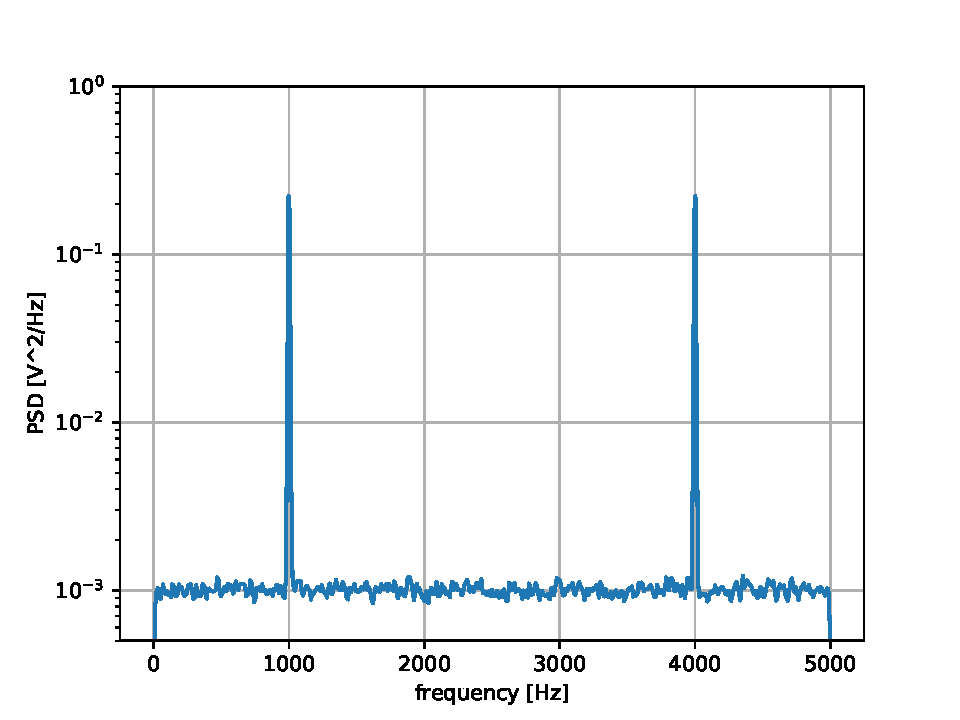
\includegraphics[width=0.9\textwidth]{figures/pwelch_1k_4k_10k}
		\caption{Densidad espectral de potencia para la suma dos senos de 1kHz y 4kHz muestreados a 10ksps}
	\end{subfigure}%
	\hspace*{10pt}
	\begin{subfigure}[t]{0.5\textwidth}
		\centering
		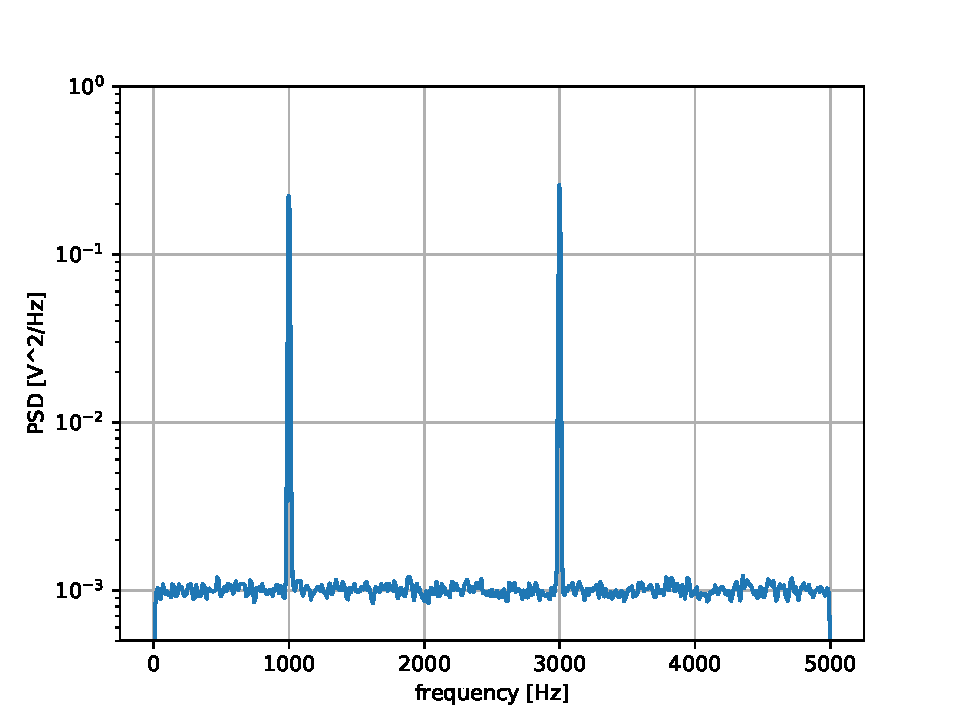
\includegraphics[width=0.9\textwidth]{figures/pwelch_1k_7k_10k}
		\caption{Densidad espectral de potencia para la suma dos senos de 1kHz y 7kHz submuestreados a 10ksps}
	\end{subfigure}
	\caption{Ejemplo de aliasing}
	\label{fig: aliasing}
\end{figure*}

En la figura \ref{fig: aliasing} se puede ver el efecto de la superposición debida al aliasing. En la primera imagen se pueden ver dos tonos a 1kHz y 4kHz respectivamente, muestreados a 10kHz. En cambio, en la segunda se ven dos tonos a 1kHz y 7kHz muestreados a 10kHz. El tono de mayor frecuencia está submuestreado por tanto los 7kHz se pliegan respecto de un eje en 5kHz apareciendo en 3kHz. De haber habido información en 3kHz ésta se hubiera superpuesto destruyendo lo que en dicha frecuencia hubiera. En la figura \ref{fig: aliasing_mirror} se muestra un esquema de lo que acaba de ocurrir, donde $\frac{f_s}{2}$ representa la mitad de la frecuencia de muestreo.

Si, la información que se encontrara más allá de la frecuencia de muestreo no fuera de interés pero no se quisiera perjudicar el ancho de banda real de la señal se debe filtrar con corte en $\frac{f_s}{2}$ para que al plegarse, el nivel de potencia sea despreciable.

\begin{figure}[ht!]
	\centering
	\resizebox{!}{!}{
		\begin{tikzpicture}
		\tikzstyle{invisible} = [outer sep=0,inner sep=0,minimum size=0]
		\tikzstyle{stealth} = [-stealth]
		\node [invisible] (v1) at (0,0) {};
		\node [invisible] (v2) at (0,2) {};
		\node [invisible] (v3) at (4.5,0) {freq};
		\draw [stealth] (v1) edge (v2);
		\draw [stealth] (v1) edge (v3);
		\draw [dashdotted](2.5,2.5) -- (2.5,-0.2) node[anchor=north]{$\frac{fs}{2}$};
		
		\draw [invisible, dotted](3.7,0) node [circle] {} -- 
		(3.5,0.8) node [circle] {} -- 
		(3.3,0) node [circle] {};
		\draw [draw](3.5,0.1) -- (3.5,-0.1) node[anchor=north]{\scriptsize$\frac{fs}{2} + \Delta f$};
		\draw [invisible](1.7,0) node [circle] {} -- 
		(1.5,0.8) node [circle] {} -- 
		(1.3,0) node [circle] {};
		\draw [draw](1.5,0.1) -- (1.5,-0.1) node[anchor=north]{\scriptsize$\frac{fs}{2} - \Delta f$};
		\draw [invisible, thick, stealth] plot[smooth, tension=.7] coordinates {(3.5,1) (2.5,1.5) (1.5,1)};
		\node [invisible, anchor=south] at (2.5,1.5) {plegado};
		\end{tikzpicture}
	}      
	\caption{Esquema del plegado de una señal con aliasing}
	\label{fig: aliasing_mirror}
\end{figure}

\subsection{Cuantización}
La cuantización consiste en obtener una señal discreta en amplitud y tiempo a partir de una señal continua en amplitud y discreta en el tiempo. Para ello, los valores de cada instante de tiempo se aproximan a los valores discretos definidos por los parámetros de la cuantización. Estos parámetros son:
\begin{itemize}
	\item \textbf{Rango dinámico [dynamic range]}. Este parámetro mide los valores máximos y mínimos hasta los cuales la señal se cuantiza. Es decir, marca los umbrales de la señal. Si los valores de la señal exceden estos límites, la señal se corta apareciendo el llamado efecto \textit{clipping}. A mayor rango dinámico para el mismo número de bits mayor rango de valores podrá obtener la señal pero con menor precisión; i.e., los saltos entre estos serán mayores.
	\item \textbf{Precisión en bits de la digitalización [\gls{ADC} number of bits]}. Este valor representa el número de escalones en los cuales se divide la escalera de cuantización. Es decir, el número de los posibles valores que puede tomar la señal digital. A mayor número de bits para el mismo rango dinámico, la precisión de la cuantización será mejor.
\end{itemize}

\begin{figure}[ht!]
	\centering
	\resizebox{!}{!}{
		\begin{tikzpicture}
		\tikzstyle{stealth} = [-stealth, thick]
		\tikzstyle{invisible} = [outer sep=0,inner sep=0,minimum size=0]
		\tikzstyle{circle} = [shape=circle, minimum size=0.5cm, draw=black!55]
		\tikzstyle{line} = [draw, very thick, red]
		\draw (-0.5,1)node[left,font=\tiny] {} -- (10.5,1);
		\draw (-0.5,-1)node[left,font=\tiny] {} -- (10.5,-1);
		\draw (-0.5,-0.33)node[left,font=\tiny] {} -- (10.5,-0.33); 
		\draw (-0.5,0.33)node[left,font=\tiny] {} -- (10.5,0.33); 
		\foreach \x in {0,0.1,0.2,0.3,0.4,0.5,0.6,0.7,0.8,0.9,1}
		{
			\draw (\x*10,-1.5)node [below,font=\tiny,] {\x } -- (\x*10,1.5) ;
		}
		\draw[ultra thick, ] (0,0) node (v5) {} sin (2.5,1) node (v7) {};
		\draw[ultra thick, ] (2.5,1) cos (5,0) node (v9) {};
		\draw[ultra thick, ] (5,0) sin (7.5,-1) node (v11) {};
		\draw[ultra thick, ] (7.5,-1) cos (10,0) node (v13) {};
		
		\node [invisible] (v1) at (-0.5,-1.5) {};
		\node [invisible] (v2) at (-0.5,2) {amplitud};
		\node [invisible] (v3) at (11,-1.5) {tiempo};
		\draw [stealth] (v1) edge (v2);
		\draw [stealth] (v1) edge (v3);
		\node [circle] (v4) at (0,-0.33) {};
		\node [circle] (v6) at (1,0.33) {};
		\node [circle] (v8) at (2,1) {};
		\node [circle] (v10) at (3,1) {};
		\node [circle] (v12) at (4,0.33) {};
		\node [circle] (v14) at (5,-0.33) {};
		\node [circle] at (6,-0.33) {};
		\node [circle] (v15) at (7,-1) {};
		\node [circle] at (8,-1) {};
		\node [circle] (v16) at (9,-0.33) {};
		\node [circle] (v17) at (10,-0.33) {};
		\draw [line](0,-0.33) -- (1,-0.33) node [invisible] {} -- (1,0.33) -- 
		(2,0.33) node [invisible] {} -- (2,1) -- 
		(4,1) node [invisible] {} -- (4,0.33) -- 
		(5,0.33) node [invisible] {} -- (5,-0.33) -- 
		(7,-0.33) node [invisible] {} -- (7,-1) -- 
		(9,-1) node [invisible] {} -- (9,-0.33) -- (10,-0.33);
		\end{tikzpicture}
	}      
	\caption{Esquema de la cuantización con 2 bits a 10 muestras por segundo, i.e., 4 valores posibles}
	\label{fig: cuantization_2bit}
\end{figure}

\begin{figure}[ht!]
	\centering
	\resizebox{!}{!}{
		\begin{tikzpicture}
		\tikzstyle{stealth} = [-stealth, thick]
		\tikzstyle{invisible} = [outer sep=0,inner sep=0,minimum size=0]
		\tikzstyle{circle} = [shape=circle, minimum size=0.5cm, draw=black!55]
		\tikzstyle{line} = [draw, very thick, red]
		\draw (-0.5,1)node[left,font=\tiny] {} -- (10.5,1);
		\draw (-0.5,0.7142)node[left,font=\tiny] {} -- (10.5,0.7142);
		\draw (-0.5,0.4285)node[left,font=\tiny] {} -- (10.5,0.4285);
		\draw (-0.5,0.1428)node[left,font=\tiny] {} -- (10.5,0.1428);
		\draw (-0.5,-0.1428)node[left,font=\tiny] {} -- (10.5,-0.1428);
		\draw (-0.5,-0.4285)node[left,font=\tiny] {} -- (10.5,-0.4285);
		\draw (-0.5,-0.7142)node[left,font=\tiny] {} -- (10.5,-0.7142);
		\draw (-0.5,-1)node[left,font=\tiny] {$y=-1$} -- (10.5,-1);
		\foreach \x in {0,0.1,0.2,0.3,0.4,0.5,0.6,0.7,0.8,0.9,1}
		{
			\draw (\x*10,-1.5)node [below,font=\tiny,] {\x } -- (\x*10,1.5) ;
		}
		\draw[ultra thick, ] (0,0) node (v5) {} sin (2.5,1) node (v7) {};
		\draw[ultra thick, ] (2.5,1) cos (5,0) node (v9) {};
		\draw[ultra thick, ] (5,0) sin (7.5,-1) node (v11) {};
		\draw[ultra thick, ] (7.5,-1) cos (10,0) node (v13) {};
		
		\node [invisible] (v1) at (-0.5,-1.5) {};
		\node [invisible] (v2) at (-0.5,2) {amplitud};
		\node [invisible] (v3) at (11,-1.5) {tiempo};
		\draw [stealth] (v1) edge (v2);
		\draw [stealth] (v1) edge (v3);
		\node [circle] (v4) at (0,0.1428) {};
		\node [circle] (v6) at (1,0.7142) {};
		\node [circle] (v8) at (2,1) {};
		\node [circle] (v10) at (3,1) {};
		\node [circle] (v12) at (4,0.7) {};
		\node [circle] (v14) at (5,0.1) {};
		\node [circle] at (6,-0.7) {};
		\node [circle] (v15) at (7,-1) {};
		\node [circle] at (8,-1) {};
		\node [circle] (v16) at (9,-0.7) {};
		\node [circle] (v17) at (10,0) {};
		\draw [line](0,0.1428) -- (1,0.1428) node [invisible] {} -- (1,0.7) -- 
		(2,0.7) node [invisible] {} -- (2,1) -- 
		(4,1) node [invisible] {} -- (4,0.7) -- 
		(5,0.7) node [invisible] {} -- (5,0.1) node [invisible] {} --
		(6,0.1) -- (6,-0.7) node [invisible] {} --
		(7,-0.7) node [invisible] {} -- (7,-1) -- 
		(9,-1) node [invisible] {} -- (9,-0.7) -- (10,-0.7) -- (10,-0.14);
		\end{tikzpicture}
	}      
	\caption{Esquema de la cuantización con 4 bits a 10 muestras por segundo, i.e., 8 valores posibles}
	\label{fig: cuantization_4bit}
\end{figure}

En las figuras \ref{fig: cuantization_2bit} y \ref{fig: cuantization_4bit} se pueden ver ejemplos de una cuantización con 2 y 4 bits respectivamente.

\begin{figure}[ht!]
	\centering
	\resizebox{!}{!}{
		\begin{tikzpicture}
		\tikzstyle{stealth} = [-stealth, thick]
		\tikzstyle{invisible} = [outer sep=0,inner sep=0,minimum size=0]
		\tikzstyle{circle} = [shape=circle, minimum size=0.5cm, draw=black!55]
		\tikzstyle{line} = [draw, very thick, red]
		
		\draw (0,0) node [invisible] (v1) {} --
		(4,0) node [invisible] {} --
		(4,4) node [invisible] {} --
		(0,4) node [invisible] {} --
		(0,0) node [invisible] {};
		\foreach \x in {0,0.25,0.5,0.75,1}
		{
			\draw (\x*4,-0.1)node [below,font=\tiny,] {\x } -- (\x*4,0.1) ;
		}
		\foreach \x in {0.125,0.375,0.625,0.875,1}
		{
			\draw (\x*4,-0.1)node [below,font=\tiny,] {} -- (\x*4,0.1);
		}
		\foreach \c [count=\x from 0] in {{000},{001},{010},{011},{100},{101},{110},{111}}
		{
			\draw (-0.1,\x*0.5)node [anchor=east,font=\tiny,] {\c} -- (0.1,\x*0.5);
		}
		%\node at (0,\x) {\c};	
		\draw [line](v1) -- (0.25,0) node [invisible] {} -- 
		(0.25,0.5) node [invisible] {} -- 
		(0.75,0.5) node [invisible] {} -- 
		(0.75,1) node [invisible] {} -- 
		(1.25,1) node [invisible] {} -- 
		(1.25,1.5) node [invisible] {} -- 
		(1.75,1.5) node [invisible] {} -- 
		(1.75,2) node [invisible] {} -- 
		(2.25,2) node [invisible] {} -- 
		(2.25,2.5) node [invisible] {} -- 
		(2.75,2.5) node [invisible] {} -- 
		(2.75,3) node [invisible] {} -- 
		(3.25,3) node [invisible] {} -- 
		(3.25,3.5) node [invisible] {} -- 
		(4,3.5) node [invisible] {};
		\node [invisible] at (2.0187,-1) {$(V_{in}-V_{RefLo})/E_{FSR}$};
		\node [invisible, rotate=90] at (-0.8509,1.9232) {$ADC_{code}$};
		\draw [dashed](0,2) node [invisible] {} -- (2,2) node [invisible] {} -- (2,0) node [invisible] {};
		\draw [dashed](0,3.5) node [invisible] {} -- (3.5,3.5) node [invisible] {} -- (3.5,0) node [invisible] {};
		\draw [dashed](0.25,4) node [] {} -- (0.25,-0.25) node [anchor=north] {\tiny LSB};
		\end{tikzpicture}
	}      
	\caption{Resolución del \gls{ADC}}
	\label{fig: adc_resolution}
\end{figure}

En la figura \ref{fig: adc_resolution} se muestra la escalera de cuantización con la resolución del \gls{ADC} calculada como se muestra en \ref{eq: adc_resolution}
\begin{align}
Q&=\frac{E_{FSR}}{2^M}\text{ donde,} \\ \nonumber
E_{FSR}&= V_{RefHi}\text{-}V_{RefLow} \\ \nonumber
\text{siendo }&V_{RefHi}\text{ el voltaje máximo de referencia}\\ \nonumber
&V_{RefLow}\text{ el voltaje mínimo de referencia y}\\ \nonumber
&M\text{ el número de bits de precisión}
\end{align}\label{eq: adc_resolution}

\section{Proceso tradicional vs redes neuronales}
El proceso tradicional consiste en procesar la señal digital con técnicas de \gls{DSP}. Estas técnicas pueden ser de muchos tipos y aplicadas tanto en el dominio del tiempo como en el dominio de la frecuencia. Este tipo de procesado es muy efectivo pero tiene el inconveniente de que si no está lo bastante adaptado para el problema en cuestión, destruye información válida en lugar de limpiar el ruido. Este proceso de afinado \textit{fine tuning} es una tarea tediosa y no siempre aplica del mismo modo dado que pequeñas variaciones en el entorno hacen que haya que tunear de nuevo la cadena de procesado de señal.

En contrapartida, están las redes neuronales que, siendo entrenadas con un gran abanico de señales y de ruidos pueden aprender a discernir patrones para limpiar así las señales del ruido. Estos algoritmos son computacionalmente costosos en comparación al \gls{DSP} tradicional. Es por ello que algunos autores han realizado sistemas híbridos en los cuales el procesado se hace con \gls{DSP} y el tuneo fino con redes neuronales. De este modo, se obtienen buenas características de ambos, pero sigue existiendo la limitación del procesado tradicional de \gls{DSP} que se limita a la cadena de procesado programada, i.e., las etapas de procesado son estáticas en diseño o su morfología no se adapta según las variaciones del entorno.

\section{Redes neuronales para series temporales}
Una serie temporal es una sucesión de valores que representan una magnitud variable con el tiempo. En el caso de sonido es una onda de presión. En las series temporales, las muestras están relacionadas con su predecesoras y afectarán a sus sucesoras. Las redes neuronales tradicionales no tienen en cuenta los estados anteriores. En el ejemplo de un clasificador de imágenes, la imagen anterior no está relacionada con la siguiente, es decir, la imagen $i$ puede ser un perro y la $i+1$ un gato pero no existe ninguna relación entre la secuencia de imágenes; hay que aclarar que el caso de un vídeo es diferente porque los fotogramas si guardan relación entre ellos.

Esto demuestra que hace falta algún tipo de neurona o entidad que tenga memoria y sea capaz de relacionar los estados anteriores con los posteriores. Este hecho dio lugar a las \textbf{redes neuronales recurrentes}. Es importante remarcar que, el hecho de que tenga memoria implica que, internamente, tiene un estado y para las mismas entradas las salidas pueden ser diferentes debido a que este estado cambie. La imagen \ref{fig: nn_vs_rnn} se puede ver una esquema de cómo las neuronas recurrentes son afectadas por su estado o salida anterior.

\begin{figure}[ht!]
	\centering
	\resizebox{!}{!}{
		\begin{tikzpicture}
		\tikzstyle{box} = [draw,inner sep=7,minimum size=57,line 
		width=1, very thick, draw=black, fill=black!20, text width=60pt, text centered]
		\tikzstyle{stealth} = [-stealth, thick]
		\tikzstyle{invisible} = [outer sep=0,inner sep=0,minimum size=0]
		\tikzstyle{circle} = [shape=circle, minimum size=0.5cm, draw=black!55]
		\tikzstyle{line} = [draw, very thick, red]
		
		\begin{scope}
		\node [box] (v2) at (0,0) {Neurona tradicional};
		\node [circle, fill] (v1) at (0,2.5) {};
		\node [circle, fill] (v3) at (0,-2.5) {};
		\draw [stealth] (v1) edge node[anchor=east] {$x(t)$} (v2);
		\draw [stealth] (v2) edge node[anchor=east] {$y(t)$} (v3);
		\end{scope}
		\begin{scope}[shift={(3.5,0)}]
		\node [box] (v2_1) at (0,0) {Neurona recurrente};
		\node [circle, fill] (v1_1) at (0,2.5) {};
		\node [circle, fill] (v3_1) at (0,-2.5) {};
		\draw [stealth] (v1_1) edge node [anchor=east] {$x(t)$} (v2_1);
		\draw [stealth] (v2_1) edge node [anchor=east] {$y(t)$} (v3_1);
		\end{scope}
		
		\node [invisible, anchor=east] (v5) at (4.75,1.25) {};
		\draw [stealth, in =0, out=0] (v5) edge node[anchor=north west] {$h(t-1)$} (v2_1);
		\node [invisible] (v4) at (2.25,1.25) {};
		\node [] (v6) at (3.5,1.25) {};
		\draw [thick, in =180, out=180] (v2_1) edge (v4);
		\draw [thick] (v4) edge (v6);
		\draw [thick] (v6) edge (v5);
		\end{tikzpicture}
	}      
	\caption{Comparación de neuronas tradicionales con neuronas recurrentes}
	\label{fig: nn_vs_rnn}
\end{figure}

Principalmente existen dos tipos de neuronas recurrentes, las \glspl{GRU} y las \glspl{LSTM}. A continuación se detalla una explicación de las neuronas \glspl{LSTM} dado que son las usadas por este trabajo.

\subsection{\acrshort{LSTM}}
Las celdas \gls{LSTM} fueron propuestas por Sepp Hochreiter y Jürgen Schmidhuber en 1997 \cite{lstm}. Estas redes se crearon para evitar el problema de las dependencias a largo plazo. Esto es, tener en cuenta estados que ocurrieron muchas iteraciones atrás en el tiempo. De esta manera las redes compuestas por celdas \glspl{LSTM} son capaces de 'recordar' información por largos períodos de tiempo\cite{colah}.

\begin{figure}[ht!]
	\centering
	\resizebox{\textwidth}{!}{
		\begin{tikzpicture}
		\tikzstyle{box} = [draw,minimum size=15,line width=1, very thick, draw=black, fill=black!30, text centered]
		\tikzstyle{stealth} = [-stealth, thick]
		\tikzstyle{invisible} = [outer sep=0,inner sep=0,minimum size=0]
		\tikzstyle{circle} = [shape=ellipse, minimum size=15pt, draw=black!, text width=15pt, text centered]
		\tikzstyle{circle_op} = [shape=circle, minimum size=0.5cm, draw=black, very thick, fill=black!10]
		\tikzstyle{line} = [draw, very thick, red]
		\begin{scope}
		\node [circle] (v14) at (-2.25,-0.75) {$x_t$};
		\node [box] (v1) at (-1.5,0.5) {$\sigma$};
		\node [box] (v3) at (-0.5,0.5) {$\sigma$};
		\node [box] (v8) at (0.5,0.5) {$\tanh$};
		\node [box] (v6) at (1.5,0.5) {$\sigma$};
		\node [circle_op] (v2) at (-1.5,2.5) {x};
		\node [circle_op] (v4) at (0.5,1.5) {x};
		\node [circle_op] (v5) at (0.5,2.5) {\scriptsize$+$};
		\node [circle_op] (v7) at (2.5,1.25) {x};
		\node [ellipse, draw, very thick, fill=black!10] (v13) at (2.5,2) {$\tanh$};
		\draw [stealth] (v1) edge (v2);
		\draw [stealth,out=90,in=180] (v3) edge (v4);
		\draw [stealth] (v4) edge (v5);
		\draw [stealth,out=90,in=180] (v6) edge (v7);
		\node [invisible] (v11) at (-2,0) {};
		\node [invisible] (v10) at (-0.5,0) {};
		\node [invisible] (v9) at (0.5,0) {};
		\node [invisible] (v12) at (1,0) {};
		\draw [thick] (v8) edge (v4);
		\draw [thick,] (v9) edge (v8);
		\draw [thick] (v10) edge (v3);
		\draw [thick] (v11) edge (v12);
		\draw [thick,out=0,in=270] (v12) edge (v6);
		\draw [thick] (v7) edge (v13);
		\draw [thick] (v2) edge (v5);
		\draw [thick,out=90,in=180] (v14) edge (v11);
		\draw [thick,out=0,in=270] (v11) edge (v1);
		\node [invisible] (v22) at (-2.75,0) {};
		\node [invisible] (v21) at (-2.75,2.5) {};
		\node [invisible] (v17) at (4,2.5) {};
		\node [circle] (v19) at (3.5,4) {$h_t$};
		\node [invisible] (v16) at (4,0) {};
		\node [invisible] (v15) at (3,0) {};
		\draw [stealth] (v15) edge (v16);
		\draw [stealth] (v5) edge (v17);
		\node (v18) at (3.5,2.5) {};
		\draw [stealth] (v18) edge (v19);
		\node [invisible] (v20) at (3.5,0) {};
		\draw [thick] (v20) edge (v18);
		\draw [thick,out=270,in=180] (v7) edge (v15);
		\draw [thick] (v21) edge (v2);
		\draw [thick] (v22) edge (v11);
		\node [invisible] (v23) at (2.5,2.5) {};
		\draw [thick] (v13) edge (v23);
		\draw [rounded corners=2ex] (-2.75,3) rectangle (3.75,-0.25);
		\end{scope}
		\begin{scope}[shift={(6.75,0)}]
		\node [circle] (v14) at (-2.25,-0.75) {$x_{t+1}$};
		\node [box] (v1) at (-1.5,0.5) {$\sigma$};
		\node [box] (v3) at (-0.5,0.5) {$\sigma$};
		\node [box] (v8) at (0.5,0.5) {$\tanh$};
		\node [box] (v6) at (1.5,0.5) {$\sigma$};
		\node [circle_op] (v2) at (-1.5,2.5) {x};
		\node [circle_op] (v4) at (0.5,1.5) {x};
		\node [circle_op] (v5) at (0.5,2.5) {\scriptsize$+$};
		\node [circle_op] (v7) at (2.5,1.25) {x};
		\node [ellipse, draw, very thick, fill=black!10] (v13) at (2.5,2) {$\tanh$};
		\draw [stealth] (v1) edge (v2);
		\draw [stealth,out=90,in=180] (v3) edge (v4);
		\draw [stealth] (v4) edge (v5);
		\draw [stealth,out=90,in=180] (v6) edge (v7);
		\node [invisible] (v11) at (-2,0) {};
		\node [invisible] (v10) at (-0.5,0) {};
		\node [invisible] (v9) at (0.5,0) {};
		\node [invisible] (v12) at (1,0) {};
		\draw [thick] (v8) edge (v4);
		\draw [thick,] (v9) edge (v8);
		\draw [thick] (v10) edge (v3);
		\draw [thick] (v11) edge (v12);
		\draw [thick,out=0,in=270] (v12) edge (v6);
		\draw [thick] (v7) edge (v13);
		\draw [thick] (v2) edge (v5);
		\draw [thick,out=90,in=180] (v14) edge (v11);
		\draw [thick,out=0,in=270] (v11) edge (v1);
		\node [invisible] (v22) at (-2.75,0) {};
		\node [invisible] (v21) at (-2.75,2.5) {};
		\node [invisible] (v17) at (4,2.5) {};
		\node [circle] (v19) at (3.5,4) {$h_{t+1}$};
		\node [invisible] (v16) at (4,0) {};
		\node [invisible] (v15) at (3,0) {};
		\draw [stealth] (v15) edge (v16);
		\draw [stealth] (v5) edge (v17);
		\node (v18) at (3.5,2.5) {};
		\draw [stealth] (v18) edge (v19);
		\node [invisible] (v20) at (3.5,0) {};
		\draw [thick] (v20) edge (v18);
		\draw [thick,out=270,in=180] (v7) edge (v15);
		\draw [thick] (v21) edge (v2);
		\draw [thick] (v22) edge (v11);
		\node [invisible] (v23) at (2.5,2.5) {};
		\draw [thick] (v13) edge (v23);
		\draw [rounded corners=2ex,fill=black!60,opacity=0.8] (-2.75,3) rectangle (3.75,-0.25);
		\end{scope}
		\begin{scope}[shift={(-6.75,0)}]
		\node [circle] (v14) at (-2.25,-0.75) {$x_{t-1}$};
		\node [box] (v1) at (-1.5,0.5) {$\sigma$};
		\node [box] (v3) at (-0.5,0.5) {$\sigma$};
		\node [box] (v8) at (0.5,0.5) {$\tanh$};
		\node [box] (v6) at (1.5,0.5) {$\sigma$};
		\node [circle_op] (v2) at (-1.5,2.5) {x};
		\node [circle_op] (v4) at (0.5,1.5) {x};
		\node [circle_op] (v5) at (0.5,2.5) {\scriptsize$+$};
		\node [circle_op] (v7) at (2.5,1.25) {x};
		\node [ellipse, draw, very thick, fill=black!10] (v13) at (2.5,2) {$\tanh$};
		\draw [stealth] (v1) edge (v2);
		\draw [stealth,out=90,in=180] (v3) edge (v4);
		\draw [stealth] (v4) edge (v5);
		\draw [stealth,out=90,in=180] (v6) edge (v7);
		\node [invisible] (v11) at (-2,0) {};
		\node [invisible] (v10) at (-0.5,0) {};
		\node [invisible] (v9) at (0.5,0) {};
		\node [invisible] (v12) at (1,0) {};
		\draw [thick] (v8) edge (v4);
		\draw [thick,] (v9) edge (v8);
		\draw [thick] (v10) edge (v3);
		\draw [thick] (v11) edge (v12);
		\draw [thick,out=0,in=270] (v12) edge (v6);
		\draw [thick] (v7) edge (v13);
		\draw [thick] (v2) edge (v5);
		\draw [thick,out=90,in=180] (v14) edge (v11);
		\draw [thick,out=0,in=270] (v11) edge (v1);
		\node [invisible] (v22) at (-2.75,0) {};
		\node [invisible] (v21) at (-2.75,2.5) {};
		\node [invisible] (v17) at (4,2.5) {};
		\node [circle] (v19) at (3.5,4) {$h_{t-1}$};
		\node [invisible] (v16) at (4,0) {};
		\node [invisible] (v15) at (3,0) {};
		\draw [stealth] (v15) edge (v16);
		\draw [stealth] (v5) edge (v17);
		\node (v18) at (3.5,2.5) {};
		\draw [stealth] (v18) edge (v19);
		\node [invisible] (v20) at (3.5,0) {};
		\draw [thick] (v20) edge (v18);
		\draw [thick,out=270,in=180] (v7) edge (v15);
		\draw [thick] (v21) edge (v2);
		\draw [thick] (v22) edge (v11);
		\node [invisible] (v23) at (2.5,2.5) {};
		\draw [thick] (v13) edge (v23);
		\draw [rounded corners=2ex,fill=black!60,opacity=0.8] (-2.75,3) rectangle (3.75,-0.25);
		\end{scope}
		\end{tikzpicture}
	}      
	\caption{Celdas \glspl{LSTM}}
	\label{fig: lstm}
\end{figure}

En la figura \ref{fig: lstm} se pueden ver tres módulos \glspl{LSTM} conectados. El diagrama contiene varias entidades:
\begin{itemize}
	\item $x_t$ representan las entradas en los diferentes instantes de tiempo; estas entradas son los vectores de entrada, dado que cada línea contiene un vector completo.
	\item $h_t$ representan las salidas. 
	\item Las operaciones en círculo o elipse son operaciones elemento a elemento de un vector respecto del otro.
	\item Los rectángulos representan capas de redes neuronales.
	\item Las líneas que se juntas representan concatenaciones de vector.
	\item Las líneas que divergen representan copias del vector por cada línea.
\end{itemize}

\begin{figure}[ht!]
	\centering
	\resizebox{!}{!}{
		\begin{tikzpicture}
		\tikzstyle{box} = [draw,minimum size=15,line width=1, very thick, draw=black, fill=black!30, text centered]
		\tikzstyle{stealth} = [-stealth, thick]
		\tikzstyle{invisible} = [outer sep=0,inner sep=0,minimum size=0]
		\tikzstyle{circle} = [shape=ellipse, minimum size=15pt, draw=black!, text width=15pt, text centered]
		\tikzstyle{circle_op} = [shape=circle, minimum size=0.5cm, draw=black, very thick, fill=black!10]
		\tikzstyle{line} = [draw, very thick, red]
		\begin{scope}
		\node [circle] (v14) at (-2.25,-0.75) {$x_t$};
		\node [box] (v1) at (-1.5,0.5) {$\sigma$};
		\node [box] (v3) at (-0.5,0.5) {$\sigma$};
		\node [box] (v8) at (0.5,0.5) {$\tanh$};
		\node [box] (v6) at (1.5,0.5) {$\sigma$};
		\node [circle_op] (v2) at (-1.5,2.5) {x};
		\node [circle_op] (v4) at (0.5,1.5) {x};
		\node [circle_op] (v5) at (0.5,2.5) {\scriptsize$+$};
		\node [circle_op] (v7) at (2.5,1.25) {x};
		\node [ellipse, draw, very thick, fill=black!10] (v13) at (2.5,2) {$\tanh$};
		\draw [stealth] (v1) edge (v2);
		\draw [stealth,out=90,in=180] (v3) edge (v4);
		\draw [stealth] (v4) edge (v5);
		\draw [stealth,out=90,in=180] (v6) edge (v7);
		\node [invisible] (v11) at (-2,0) {};
		\node [invisible] (v10) at (-0.5,0) {};
		\node [invisible] (v9) at (0.5,0) {};
		\node [invisible] (v12) at (1,0) {};
		\draw [thick] (v8) edge (v4);
		\draw [thick,] (v9) edge (v8);
		\draw [thick] (v10) edge (v3);
		\draw [thick] (v11) edge (v12);
		\draw [thick,out=0,in=270] (v12) edge (v6);
		\draw [thick] (v7) edge (v13);
		\draw [thick] (v2) edge (v5);
		\draw [thick,out=90,in=180] (v14) edge (v11);
		\draw [thick,out=0,in=270] (v11) edge (v1);
		\node [invisible] (v22) at (-3.5,0) {$h_{t-1}$};
		\node [invisible] (v21) at (-3.5,2.5) {$C_{t-1}$};
		\node [invisible] (v17) at (4.5,2.5) {$C_{t}$};
		\node [circle] (v19) at (3.5,4) {$h_t$};
		\node [invisible] (v16) at (4.5,0) {$h_{t}$};
		\node [invisible] (v15) at (3,0) {};
		\draw [stealth] (v15) edge (v16);
		\draw [stealth] (v5) edge (v17);
		\node (v18) at (3.5,2.5) {};
		\draw [stealth] (v18) edge (v19);
		\node [invisible] (v20) at (3.5,0) {};
		\draw [thick] (v20) edge (v18);
		\draw [thick,out=270,in=180] (v7) edge (v15);
		\draw [thick] (v21) edge (v2);
		\draw [thick] (v22) edge (v11);
		\node [invisible] (v23) at (2.5,2.5) {};
		\draw [thick] (v13) edge (v23);
		\draw [rounded corners=2ex] (-2.75,3) rectangle (3.75,-0.25);
		\end{scope}
		\fill [white,opacity=0.7]  (-4,4.5) rectangle (5,-1.5);
		\node [invisible] (V_cneg) at (-3.5,2.5) {$C_{t-1}$};
		\node [invisible] (V_cpos) at (4.5,2.5) {$C_{t}$};
		\node [circle_op] (v5) at (0.5,2.5) {\scriptsize$+$};
		\node [circle_op] (v2) at (-1.5,2.5) {x};
		\draw [thick] (v21) edge (v2);
		\draw [thick] (v2) edge (v5);
		\draw [stealth] (v5) edge (v17);
		\end{tikzpicture}
	}      
	\caption{Propagación del estado de una celda \gls{LSTM}}
	\label{fig: lstm_state}
\end{figure}

La línea superior de la celda se propaga a lo largo de todas las celdas de la cadena como se muestra en la figura \ref{fig: lstm_state}.

Las celdas tienen la capacidad de eliminar e introducir información mediante la red de neuronas sigmoide seguida de una multiplicación elemento a elemento. La red de neuronas sigmoide da un peso entre cero y uno en función de la importancia de cada componente. A este conjunto de elementos se les llama puertas porque tienen la capacidad de dejar pasar información o no. La salida del sigmoide próxima a cero no deja pasar información, por el contrario, próxima a uno si la deja pasar.

\subsubsection{Ponderando el estado anterior}
A la entrada de la celda lo primero que aparece es la llamada capa de la puerta de olvido, en inglés, \textit{forget gate layer}. Esta puerta tiene la función de discernir cuánto del estado anterior permanece y cuánto se desecha. Como en todas las puerta la salida es entre 0 y 1 y después se multiplica por el estado anterior $C_{t-1}$. En la figura \ref{fig: lstm_forgot} se pueden ver los bloques implicados en esta operación donde la salida del sigmoide tiene el valor:

\begin{align}
	f_t = \sigma \left( W_f\cdot \left[ h_{t-1}, x_t \right] + b_f \right)
\end{align}
\vspace*{-30pt}
\begin{figure}[ht!]
	\centering
	\resizebox{!}{!}{
		\begin{tikzpicture}
		\tikzstyle{box} = [draw,minimum size=15,line width=1, very thick, draw=black, fill=black!30, text centered]
		\tikzstyle{stealth} = [-stealth, thick]
		\tikzstyle{invisible} = [outer sep=0,inner sep=0,minimum size=0]
		\tikzstyle{circle} = [shape=ellipse, minimum size=15pt, draw=black!, text width=15pt, text centered]
		\tikzstyle{circle_op} = [shape=circle, minimum size=0.5cm, draw=black, very thick, fill=black!10]
		\tikzstyle{line} = [draw, very thick, red]
		\begin{scope}
		\node [circle] (v14) at (-2.25,-0.75) {$x_t$};
		\node [box] (v1) at (-1.5,0.5) {$\sigma$};
		\node [box] (v3) at (-0.5,0.5) {$\sigma$};
		\node [box] (v8) at (0.5,0.5) {$\tanh$};
		\node [box] (v6) at (1.5,0.5) {$\sigma$};
		\node [circle_op] (v2) at (-1.5,2.5) {x};
		\node [circle_op] (v4) at (0.5,1.5) {x};
		\node [circle_op] (v5) at (0.5,2.5) {\scriptsize$+$};
		\node [circle_op] (v7) at (2.5,1.25) {x};
		\node [ellipse, draw, very thick, fill=black!10] (v13) at (2.5,2) {$\tanh$};
		\draw [stealth] (v1) edge (v2);
		\draw [stealth,out=90,in=180] (v3) edge (v4);
		\draw [stealth] (v4) edge (v5);
		\draw [stealth,out=90,in=180] (v6) edge (v7);
		\node [invisible] (v11) at (-2,0) {};
		\node [invisible] (v10) at (-0.5,0) {};
		\node [invisible] (v9) at (0.5,0) {};
		\node [invisible] (v12) at (1,0) {};
		\draw [thick] (v8) edge (v4);
		\draw [thick,] (v9) edge (v8);
		\draw [thick] (v10) edge (v3);
		\draw [thick] (v11) edge (v12);
		\draw [thick,out=0,in=270] (v12) edge (v6);
		\draw [thick] (v7) edge (v13);
		\draw [thick] (v2) edge (v5);
		\draw [thick,out=90,in=180] (v14) edge (v11);
		\draw [thick,out=0,in=270] (v11) edge (v1);
		\node [invisible] (v22) at (-3.5,0) {$h_{t-1}$};
		\node [invisible] (v21) at (-3.5,2.5) {$C_{t-1}$};
		\node [invisible] (v17) at (4.5,2.5) {$C_{t}$};
		\node [circle] (v19) at (3.5,4) {$h_t$};
		\node [invisible] (v16) at (4.5,0) {$h_{t}$};
		\node [invisible] (v15) at (3,0) {};
		\draw [stealth] (v15) edge (v16);
		\draw [stealth] (v5) edge (v17);
		\node (v18) at (3.5,2.5) {};
		\draw [stealth] (v18) edge (v19);
		\node [invisible] (v20) at (3.5,0) {};
		\draw [thick] (v20) edge (v18);
		\draw [thick,out=270,in=180] (v7) edge (v15);
		\draw [thick] (v21) edge (v2);
		\draw [thick] (v22) edge (v11);
		\node [invisible] (v23) at (2.5,2.5) {};
		\draw [thick] (v13) edge (v23);
		\draw [rounded corners=2ex] (-2.75,3) rectangle (3.75,-0.25);
		\end{scope}
		\fill [white,opacity=0.7]  (-4,4.5) rectangle (5,-1.5);
		\node [box] (v1) at (-1.5,0.5) {$\sigma$};
		\draw [stealth] (v1) edge node [anchor=east] {$f_t$} (v2);
		\node [invisible] (v22) at (-3.5,0) {$h_{t-1}$};
		\draw [thick] (v22) edge (v11);
		\node [circle] (v14) at (-2.25,-0.75) {$x_t$};
		\draw [thick,out=90,in=180] (v14) edge (v11);
		\draw [thick,out=0,in=270] (v11) edge (v1);
		\end{tikzpicture}
	}      
	\caption{Puerta de olvido en la celda \gls{LSTM}}
	\label{fig: lstm_forgot}
\end{figure}

\subsubsection{Ponderando las nuevas entradas}
En siguiente paso consiste en discernir cuanta información de la actual a la entrada se propaga al estado actual de la celda. Este paso está dividido en dos etapas.

La primera etapa recibe el nombre de capa de puerta de entrada, en inglés \textit{input gate layer}. Esta puerta tiene la función de decidir cuáles de los valores del vector concatenado de entrada actual y salida anterior van a ser actualizados en el estado actual de la celda en la figura \ref{fig: lstm_input} y en la siguiente ecuación viene representado por $i_t$.

La segunda etapa consiste en una operación elemento a elemento de $\tanh$ en la cual se van a calcular los nuevos valores para cada elemento del vector. En la figura \ref{fig: lstm_input} y en la siguiente ecuación viene representado por $\widetilde{C_t}$.

\begin{align}
	i_t &= \sigma \left( W_f\cdot \left[ h_{t-1}, x_t \right] + b_i \right) \\ \nonumber
	\widetilde{C_t}&=\tanh \left( W_C\cdot \left[ h_{t-1}, x_t \right] + b_C \right)
\end{align}
\vspace*{-30pt}
\begin{figure}[ht!]
	\centering
	\resizebox{!}{!}{
		\begin{tikzpicture}
		\tikzstyle{box} = [draw,minimum size=15,line width=1, very thick, draw=black, fill=black!30, text centered]
		\tikzstyle{stealth} = [-stealth, thick]
		\tikzstyle{invisible} = [outer sep=0,inner sep=0,minimum size=0]
		\tikzstyle{circle} = [shape=ellipse, minimum size=15pt, draw=black!, text width=15pt, text centered]
		\tikzstyle{circle_op} = [shape=circle, minimum size=0.5cm, draw=black, very thick, fill=black!10]
		\tikzstyle{line} = [draw, very thick, red]
		\begin{scope}
		\node [circle] (v14) at (-2.25,-0.75) {$x_t$};
		\node [box] (v1) at (-1.5,0.5) {$\sigma$};
		\node [box] (v3) at (-0.5,0.5) {$\sigma$};
		\node [box] (v8) at (0.5,0.5) {$\tanh$};
		\node [box] (v6) at (1.5,0.5) {$\sigma$};
		\node [circle_op] (v2) at (-1.5,2.5) {x};
		\node [circle_op] (v4) at (0.5,1.5) {x};
		\node [circle_op] (v5) at (0.5,2.5) {\scriptsize$+$};
		\node [circle_op] (v7) at (2.5,1.25) {x};
		\node [ellipse, draw, very thick, fill=black!10] (v13) at (2.5,2) {$\tanh$};
		\draw [stealth] (v1) edge (v2);
		\draw [stealth,out=90,in=180] (v3) edge (v4);
		\draw [stealth] (v4) edge (v5);
		\draw [stealth,out=90,in=180] (v6) edge (v7);
		\node [invisible] (v11) at (-2,0) {};
		\node [invisible] (v10) at (-0.5,0) {};
		\node [invisible] (v9) at (0.5,0) {};
		\node [invisible] (v12) at (1,0) {};
		\draw [thick] (v8) edge (v4);
		\draw [thick,] (v9) edge (v8);
		\draw [thick] (v10) edge (v3);
		\draw [thick] (v11) edge (v12);
		\draw [thick,out=0,in=270] (v12) edge (v6);
		\draw [thick] (v7) edge (v13);
		\draw [thick] (v2) edge (v5);
		\draw [thick,out=90,in=180] (v14) edge (v11);
		\draw [thick,out=0,in=270] (v11) edge (v1);
		\node [invisible] (v22) at (-3.5,0) {$h_{t-1}$};
		\node [invisible] (v21) at (-3.5,2.5) {$C_{t-1}$};
		\node [invisible] (v17) at (4.5,2.5) {$C_{t}$};
		\node [circle] (v19) at (3.5,4) {$h_t$};
		\node [invisible] (v16) at (4.5,0) {$h_{t}$};
		\node [invisible] (v15) at (3,0) {};
		\draw [stealth] (v15) edge (v16);
		\draw [stealth] (v5) edge (v17);
		\node (v18) at (3.5,2.5) {};
		\draw [stealth] (v18) edge (v19);
		\node [invisible] (v20) at (3.5,0) {};
		\draw [thick] (v20) edge (v18);
		\draw [thick,out=270,in=180] (v7) edge (v15);
		\draw [thick] (v21) edge (v2);
		\draw [thick] (v22) edge (v11);
		\node [invisible] (v23) at (2.5,2.5) {};
		\draw [thick] (v13) edge (v23);
		\draw [rounded corners=2ex] (-2.75,3) rectangle (3.75,-0.25);
		\end{scope}
		\fill [white,opacity=0.7]  (-4,4.5) rectangle (5,-1.5);
		\node [invisible] (v22) at (-3.5,0) {$h_{t-1}$};
		\draw [thick] (v22) edge (v11);
		\node [circle] (v14) at (-2.25,-0.75) {$x_t$};
		\draw [thick,out=90,in=180] (v14) edge (v11);
		\draw [thick] (v11) edge (v9);
		\node [box] (v3) at (-0.5,0.5) {$\sigma$};
		\node [box] (v8) at (0.5,0.5) {$\tanh$};
		\draw [thick] (v10) edge (v3);
		\draw [thick] (v9) edge (v8);
		\draw [thick] (v8) edge node[anchor=west] {$\widetilde{C_t}$} (v4);
		\draw [stealth,out=90,in=180] (v3) edge node[anchor=east] {$i_t$}( v4);
		\end{tikzpicture}
	}      
	\caption{Puerta de entrada en la celda \gls{LSTM}}
	\label{fig: lstm_input}
\end{figure}


\subsubsection{Actualizando el estado de la celda}
A continuación hay que actualizar el estado de la celda. Para ello se multiplica el estado anterior por $f_t$ para olvidar la información que ya no es relevante y se suma la información nueva ponderada por $i_t$ como muestran la figura \ref{fig: lstm_update} y la siguiente ecuación.

\begin{align}
	C_{t} = f_t\cdot C_{t-1} + i_t \cdot \widetilde{C_t}
\end{align}
\vspace*{-30pt}
\begin{figure}[ht!]
	\centering
	\resizebox{!}{!}{
		\begin{tikzpicture}
		\tikzstyle{box} = [draw,minimum size=15,line width=1, very thick, draw=black, fill=black!30, text centered]
		\tikzstyle{stealth} = [-stealth, thick]
		\tikzstyle{invisible} = [outer sep=0,inner sep=0,minimum size=0]
		\tikzstyle{circle} = [shape=ellipse, minimum size=15pt, draw=black!, text width=15pt, text centered]
		\tikzstyle{circle_op} = [shape=circle, minimum size=0.5cm, draw=black, very thick, fill=black!10]
		\tikzstyle{line} = [draw, very thick, red]
		\begin{scope}
		\node [circle] (v14) at (-2.25,-0.75) {$x_t$};
		\node [box] (v1) at (-1.5,0.5) {$\sigma$};
		\node [box] (v3) at (-0.5,0.5) {$\sigma$};
		\node [box] (v8) at (0.5,0.5) {$\tanh$};
		\node [box] (v6) at (1.5,0.5) {$\sigma$};
		\node [circle_op] (v2) at (-1.5,2.5) {x};
		\node [circle_op] (v4) at (0.5,1.5) {x};
		\node [circle_op] (v5) at (0.5,2.5) {\scriptsize$+$};
		\node [circle_op] (v7) at (2.5,1.25) {x};
		\node [ellipse, draw, very thick, fill=black!10] (v13) at (2.5,2) {$\tanh$};
		\draw [stealth] (v1) edge (v2);
		\draw [stealth,out=90,in=180] (v3) edge (v4);
		\draw [stealth] (v4) edge (v5);
		\draw [stealth,out=90,in=180] (v6) edge (v7);
		\node [invisible] (v11) at (-2,0) {};
		\node [invisible] (v10) at (-0.5,0) {};
		\node [invisible] (v9) at (0.5,0) {};
		\node [invisible] (v12) at (1,0) {};
		\draw [thick] (v8) edge (v4);
		\draw [thick,] (v9) edge (v8);
		\draw [thick] (v10) edge (v3);
		\draw [thick] (v11) edge (v12);
		\draw [thick,out=0,in=270] (v12) edge (v6);
		\draw [thick] (v7) edge (v13);
		\draw [thick] (v2) edge (v5);
		\draw [thick,out=90,in=180] (v14) edge (v11);
		\draw [thick,out=0,in=270] (v11) edge (v1);
		\node [invisible] (v22) at (-3.5,0) {$h_{t-1}$};
		\node [invisible] (v21) at (-3.5,2.5) {$C_{t-1}$};
		\node [invisible] (v17) at (4.5,2.5) {$C_{t}$};
		\node [circle] (v19) at (3.5,4) {$h_t$};
		\node [invisible] (v16) at (4.5,0) {$h_{t}$};
		\node [invisible] (v15) at (3,0) {};
		\draw [stealth] (v15) edge (v16);
		\draw [stealth] (v5) edge (v17);
		\node (v18) at (3.5,2.5) {};
		\draw [stealth] (v18) edge (v19);
		\node [invisible] (v20) at (3.5,0) {};
		\draw [thick] (v20) edge (v18);
		\draw [thick,out=270,in=180] (v7) edge (v15);
		\draw [thick] (v21) edge (v2);
		\draw [thick] (v22) edge (v11);
		\node [invisible] (v23) at (2.5,2.5) {};
		\draw [thick] (v13) edge (v23);
		\draw [rounded corners=2ex] (-2.75,3) rectangle (3.75,-0.25);
		\end{scope}
		\fill [white,opacity=0.7]  (-4,4.5) rectangle (5,-1.5);
		\draw [thick] (v8) edge node[anchor=west] {$\widetilde{C_t}$} (v4);
		\draw [stealth,out=90,in=180] (v3) edge node[anchor=east] {$i_t$}( v4);
		\draw [stealth] (v1) edge node [anchor=east] {$f_t$} (v2);
		\node [invisible] (V_cneg) at (-3.5,2.5) {$C_{t-1}$};
		\node [invisible] (V_cpos) at (4.5,2.5) {$C_{t}$};
		\node [circle_op] (v5) at (0.5,2.5) {\scriptsize$+$};
		\node [circle_op] (v2) at (-1.5,2.5) {x};
		\draw [thick] (v21) edge (v2);
		\draw [thick] (v2) edge (v5);
		\draw [stealth] (v5) edge (v17);
		\node [circle_op] (v4) at (0.5,1.5) {x};
		\draw [stealth] (v4) edge (v5);
		\end{tikzpicture}
	}
	\vspace*{-10pt}
	\caption{Actualización del estado de la celda \gls{LSTM}}
	\label{fig: lstm_update}
\end{figure}

\subsubsection{Generando la salida}
Finalmente queda generar la salida de la celda. La salida se va a basar en el estado actual de la celda pero no directamente el estado. En primer lugar esta la última puerta de la celda que es la encargada de discernir que valores del vector saldrán (al igual que en todas las puertas, es una multiplicación elemento a elemento con un valor entre 0 y 1). Esta puerta dejará pasar los valores del vector de estado de la celda a los que previamente se les ha calculado la tangente hiperbólica cuyos valores de salida son -1 o 1. La siguiente ecuación y la figura \ref{fig: lstm_output} muestran dichos cálculos.
\begin{align}
	o_t &= \sigma \left( W_o\cdot \left[ h_{t-1}, x_t \right] + b_o \right) \\ \nonumber
	{h_t}&=o_t\cdot \tanh \left( C_t \right)
\end{align}
\vspace*{-35pt}
\begin{figure}[ht!]
	\centering
	\resizebox{!}{!}{
		\begin{tikzpicture}
		\tikzstyle{box} = [draw,minimum size=15,line width=1, very thick, draw=black, fill=black!30, text centered]
		\tikzstyle{stealth} = [-stealth, thick]
		\tikzstyle{invisible} = [outer sep=0,inner sep=0,minimum size=0]
		\tikzstyle{circle} = [shape=ellipse, minimum size=15pt, draw=black!, text width=15pt, text centered]
		\tikzstyle{circle_op} = [shape=circle, minimum size=0.5cm, draw=black, very thick, fill=black!10]
		\tikzstyle{line} = [draw, very thick, red]
		\begin{scope}
		\node [circle] (v14) at (-2.25,-0.75) {$x_t$};
		\node [box] (v1) at (-1.5,0.5) {$\sigma$};
		\node [box] (v3) at (-0.5,0.5) {$\sigma$};
		\node [box] (v8) at (0.5,0.5) {$\tanh$};
		\node [box] (v6) at (1.5,0.5) {$\sigma$};
		\node [circle_op] (v2) at (-1.5,2.5) {x};
		\node [circle_op] (v4) at (0.5,1.5) {x};
		\node [circle_op] (v5) at (0.5,2.5) {\scriptsize$+$};
		\node [circle_op] (v7) at (2.5,1.25) {x};
		\node [ellipse, draw, very thick, fill=black!10] (v13) at (2.5,2) {$\tanh$};
		\draw [stealth] (v1) edge (v2);
		\draw [stealth,out=90,in=180] (v3) edge (v4);
		\draw [stealth] (v4) edge (v5);
		\draw [stealth,out=90,in=180] (v6) edge (v7);
		\node [invisible] (v11) at (-2,0) {};
		\node [invisible] (v10) at (-0.5,0) {};
		\node [invisible] (v9) at (0.5,0) {};
		\node [invisible] (v12) at (1,0) {};
		\draw [thick] (v8) edge (v4);
		\draw [thick,] (v9) edge (v8);
		\draw [thick] (v10) edge (v3);
		\draw [thick] (v11) edge (v12);
		\draw [thick,out=0,in=270] (v12) edge (v6);
		\draw [thick] (v7) edge (v13);
		\draw [thick] (v2) edge (v5);
		\draw [thick,out=90,in=180] (v14) edge (v11);
		\draw [thick,out=0,in=270] (v11) edge (v1);
		\node [invisible] (v22) at (-3.5,0) {$h_{t-1}$};
		\node [invisible] (v21) at (-3.5,2.5) {$C_{t-1}$};
		\node [invisible] (v17) at (4.5,2.5) {$C_{t}$};
		\node [circle] (v19) at (3.5,4) {$h_t$};
		\node [invisible] (v16) at (4.5,0) {$h_{t}$};
		\node [invisible] (v15) at (3,0) {};
		\draw [stealth] (v15) edge (v16);
		\draw [stealth] (v5) edge (v17);
		\node (v18) at (3.5,2.5) {};
		\draw [stealth] (v18) edge (v19);
		\node [invisible] (v20) at (3.5,0) {};
		\draw [thick] (v20) edge (v18);
		\draw [thick,out=270,in=180] (v7) edge (v15);
		\draw [thick] (v21) edge (v2);
		\draw [thick] (v22) edge (v11);
		\node [invisible] (v23) at (2.5,2.5) {};
		\draw [thick] (v13) edge (v23);
		\draw [rounded corners=2ex] (-2.75,3) rectangle (3.75,-0.25);
		\end{scope}
		\fill [white,opacity=0.7]  (-4,4.5) rectangle (5,-1.5);
		\node [invisible] (v22) at (-3.5,0) {$h_{t-1}$};
		\draw [thick] (v22) edge (v11);
		\node [circle] (v14) at (-2.25,-0.75) {$x_t$};
		\draw [thick] (v11) edge (v12);
		\node [box] (v6) at (1.5,0.5) {$\sigma$};
		\draw [stealth,out=90,in=180] (v6) edge node[anchor=east] {$o_t$} (v7);
		\node [circle_op] (v7) at (2.5,1.25) {x};
		\node [ellipse, draw, very thick, fill=black!10] (v13) at (2.5,2) {$\tanh$};
		\node [invisible] (v16) at (4.5,0) {$h_{t}$};
		\node [circle] (v19) at (3.5,4) {$h_t$};
		\draw [stealth] (v20) edge (v16);		
		\draw [thick] (v23) edge (v13);
		\draw [thick] (v13) edge (v7);
		\draw [thick] (v15) edge (v20);
		\draw [thick,out=270,in=180] (v7) edge (v15);
		\draw [thick] (v20) edge (v18);
		\draw [stealth] (v18) edge (v19);
		\draw [thick,out=90,in=180] (v14) edge (v11);
		\draw [thick,out=0,in=270] (v12) edge (v6);
		\end{tikzpicture}
	}
	\vspace*{-10pt}
	\caption{Puerta de olvido en la celda \gls{LSTM}}
	\label{fig: lstm_output}
\end{figure}

\section{Estado del arte en cancelación de ruido con redes neuronales}
	\clearpage
	\chapter{Obtención, procesado y almacenamiento de los datos} \label{cp: dataGathering}
En este capítulo se abarca cómo se han obtenido los datos, cómo han sido almacenados y preprocesados para su explotación.

Los datos de conversaciones limpias de ruido no son algo fácil de conseguir. Son archivos que ocupan mucho disco y no se encontraron repositorios con la cantidad de información necesaria. Por otro lado está la obtención de ruidos, esta tarea si es más sencilla dado que existe gran diversidad de formas de descargarlos para sumarlos con los audios libres de ruido.

\section{Audio}
En primer lugar cabe destacar que se tuvieron en cuenta varias posibilidades durante dicha fase. A continuación se describen haciendo hincapié en la opción elegida.

\subsection{Extracción audio de YouTube}
La primera opción que se tuvo en cuenta fue la extracción del audio de videos alojados en \textbf{YouTube} de entrevistas y programas radiofónicos. Este tipo de fuentes conlleva el problema de que no se sabe a priori cuánto libres de ruidos están los audios. Usualmente, se introducen efectos o el ruido del público puede interferir el entrenamiento. Para evitar este problema habría que analizar todos los audios descargados, tarea tediosa y que requiere mucho tiempo.

\subsection{Generación de audio sintético}
La segunda opción que se barajó fue la generación de audio sintético. La generación de datos sintéticos es una técnica muy usada en el entrenamiento de modelos de \gls{ML}. Existen dos grupos en la generación de datos sintéticos:
\begin{itemize}
	\item \textbf{A partir de datos existentes}. Estas técnicas son muy usadas en el análisis de imágenes. Es muy típico ampliar el \MakeLowercase{\gls{dataset}} de imágenes para clasificadores aplicando transformaciones a la imágenes. Por ejemplo, si se está diseñando un clasificador de tipos de imágenes, una forma de ampliar el \gls{dataset} sería generar imágenes espejo de la originales. Esto consiste simplemente ordenar las columnas de la matriz de forma opuesta.
	\item \textbf{Desde cero}. Estas técnicas requieren usualmente de una red neuronal o algoritmo previamente entrenada que sea capaz de generar dichos datos de manera que sean prácticamente igual a unos reales.
\end{itemize}

En el caso del audio no se puede partir de un audio para modificarlo y expandir el \gls{dataset}. La única forma sería aplicar una ganancia en cuyo caso sería igual a subir o bajar el volumen, pero no es técnicamente generar datos nuevos. Por esta razón se eligió la segunda forma de generar datos sintéticos.

En el caso del audio, los sintetizadores existen hace mucho tiempo. Los dispositivos \gls{GPS} de los automóviles tienen un sintetizador que reproduce una voz hablada. Estos sintetizadores son algo realmente complicado de hacer y típicamente tienen voces metálicas que no reproducen fielmente una voz humana. De hecho éste es un gran campo dentro de las redes neuronales profundas. Estos tipos de algoritmo se denominan \textit{text to speech}.

Para este trabajo se desplegó el algoritmo \textit{\href{https://github.com/CorentinJ/Real-Time-Voice-Cloning}{Real Time Voice Cloning}}. Este algoritmo es un proyecto de código abierto que consiste en una red neuronal para la clonación de voz\cite{transfer_learning}. El algoritmo se entrena con una voz y después es capaz de reproducir audio con dicha voz a partir de texto.

Finalmente, tras un breve entrenamiento de esta red, se descartó debido a que los resultados generaban una voz metálica. Esto es debido al corto entrenamiento al que fue sometida la red. Cabe destacar que es un algoritmo costoso que, corriendo en gráfica dedicada tarda en generar el audio pero es un algoritmo con gran futuro y fuertemente apoyado por la comunidad open-source.

\subsection{Descarga masiva de audiolibros}
Los audiolibros son una fuente de audio en la cual no deben existir ruidos externos que afecten a la grabación, adicionalmente, son grabaciones reales de personas y se tiene mucha información adicional como el texto que se está leyendo. Por estas razones son fuentes muy válidas para entrenar redes neuronales relacionadas con el análisis de la voz humana.

Como contrapartida está que la mayoría de los audiolibros son de pago y no están disponibles para una descarga masiva. Afortunadamente, existen diferentes sitios web que almacenan audios libros de dominio público, una de las más conocidas es \href{https://librivox.org/}{Librivox}. Esta web posee audiolibros en varios idiomas perfectamente clasificados y con gran cantidad de información sobre los mismos. Adicionalmente, cuenta con una \gls{API} que consiste en un servicio web que recibe peticiones \gls{GET} y devuelve en formato \gls{HTML} o \gls{JSON} la información solicitada. Este servicio web fue probado pero los resultados no fueron los esperados dado que cuando se aplicaban los filtros, la información devuelta por el servicio no cumplía las restricciones impuestas. Como consecuencia se descartó este método de obtención de la información y las \glspl{URL} de descarga de los libros. En su lugar, se planteó el desarrollo de un algoritmo de \gls{scraper}.

Los algoritmos de \gls{scraper} son altamente utilizados para la extracción de información de manera masiva y automatizada de los sitios web. Cuando se hace una petición a un sitio web éste devuelve el código de la página web que está almacenado en el servidor que proporciona el servicio de almacenamiento web, en inglés, \textit{hosting} y el navegador web lo interpreta mostrando su contenido. La figura \ref{fig: web_nav} presenta un esquema resumido de esta comunicación. Este código puede ser analizado por un algoritmo para extraer información, salvo que el código de la página haya sido ofuscado, dado que es un código altamente estructurado. Este tipo de técnicas están en la frontera de la ética dado que también pueden ser usadas para hackeo web.

\begin{figure}[ht!]
	\centering
	\resizebox{!}{!}{
		\begin{tikzpicture}
		\tikzstyle{box} = [draw,inner sep=7,minimum size=57,line 
		width=1, very thick, draw=black, fill=black!20, text width=80, text centered]
		\tikzstyle{invisible} = [outer sep=0,inner sep=0,minimum size=0]
		\tikzstyle{stealth} = [-stealth]
		\node [box] (v1) at (0,0) {Navegador Web};
		\node [box] (v2) at (5.5,0) {Servidor de almacenamiento};
		
		\draw [stealth, in=90, out=90, very thick] (v1) edge node [anchor=south] {Petición HTTP}(v2);
		\draw [stealth, in=270, out=270, very thick] (v2) edge node [anchor=north] {Respuesta HTTP} (v1);
		\end{tikzpicture}
	}      
	\caption{Esquema de la navegación web}
	\label{fig: web_nav}
\end{figure}

Las técnias de \gls{scraper} están compuestas por varios pasos:
\begin{itemize}
	\item Exploración visual del sitio web.
	\item Análisis de la \gls{URL}. En muchas ocasiones, parte de la información que el sitio web devuelve viene filtrada mediante una serie de filtros que se definen en la \gls{URL}.
	\item Análisis del sitio web mediante herramientas de desarrollador. Consiste analizar el sitio web para encontrar dónde está la información que se quiere extraer y cómo viene en el código de la página. Para esto se usa un navegador web y se analiza el código mediante el inspector del navegador. Esta herramienta resalta cada una de las partes del código de la página web que se corresponden con las partes visuales de la misma.
	\item Extracción y almacenamiento de la información.
\end{itemize}

Existen dos tipos principales de \gls{scraper} en función del tipo de web a la que se le quiera extraer la información y del tipo de seguridad que lleve implementada:
\begin{itemize}
	\item Sitios web estáticos. Extracción con peticiones librerías de peticiones web y respuestas en código \gls{HTML}
	\item Sitio web dinámicos. Extracción avanzado mediante un driver de navegador (Firefox, Chrome\dots) y respuestas de código JavaScript.
\end{itemize}
El primero de los tipos consiste en hacer peticiones a la \gls{URL} objetivo y extraer la información devuelta en la petición. Este tipo de algoritmos no permiten hacer una navegación interactiva por la página y no permite interactuar con JavaScript, algo cada vez más presenta en las webs actuales. Como punto a favor, estos tipos de algoritmo son muy rápidos y fáciles de desarrollar. En contra partida, si se hace un número grande de peticiones al servidor éste puede bloquear la IP de entrada de la petición para protegerse de ataques.

El segundo tipo consiste en la emulación de la navegación humana llamando al navegador. Estas técnicas son mucho más avanzadas y permiten obtener información de cualquier página, rellenar formularios y hacer uso de la página como si de un humano se tratara. Aporta muchas más posibilidades que el otro tipo de \gls{scraper} y es mucho más robusto a bloqueos por parte del servidor, esto se puede mejorar incluso, poniendo esperas aleatorias entre peticiones. Sin embargo, ejecuta un navegador y, por consiguiente, es mucho más lenta la extracción de la información.

\subsubsection{Exploración visual}
Para el caso concreto del trabajo, la web objetivo se puede ver que contiene diferentes formas de analizar el catálogo. Esto no son más que filtros que se le pueden aplicar a la base de datos donde la página almacena la información. En la figura \ref{fig: librivox_cover} se puede ver la estructura de la página.
\begin{figure}[ht!]
	\centering
	\resizebox{\textwidth}{!}{
		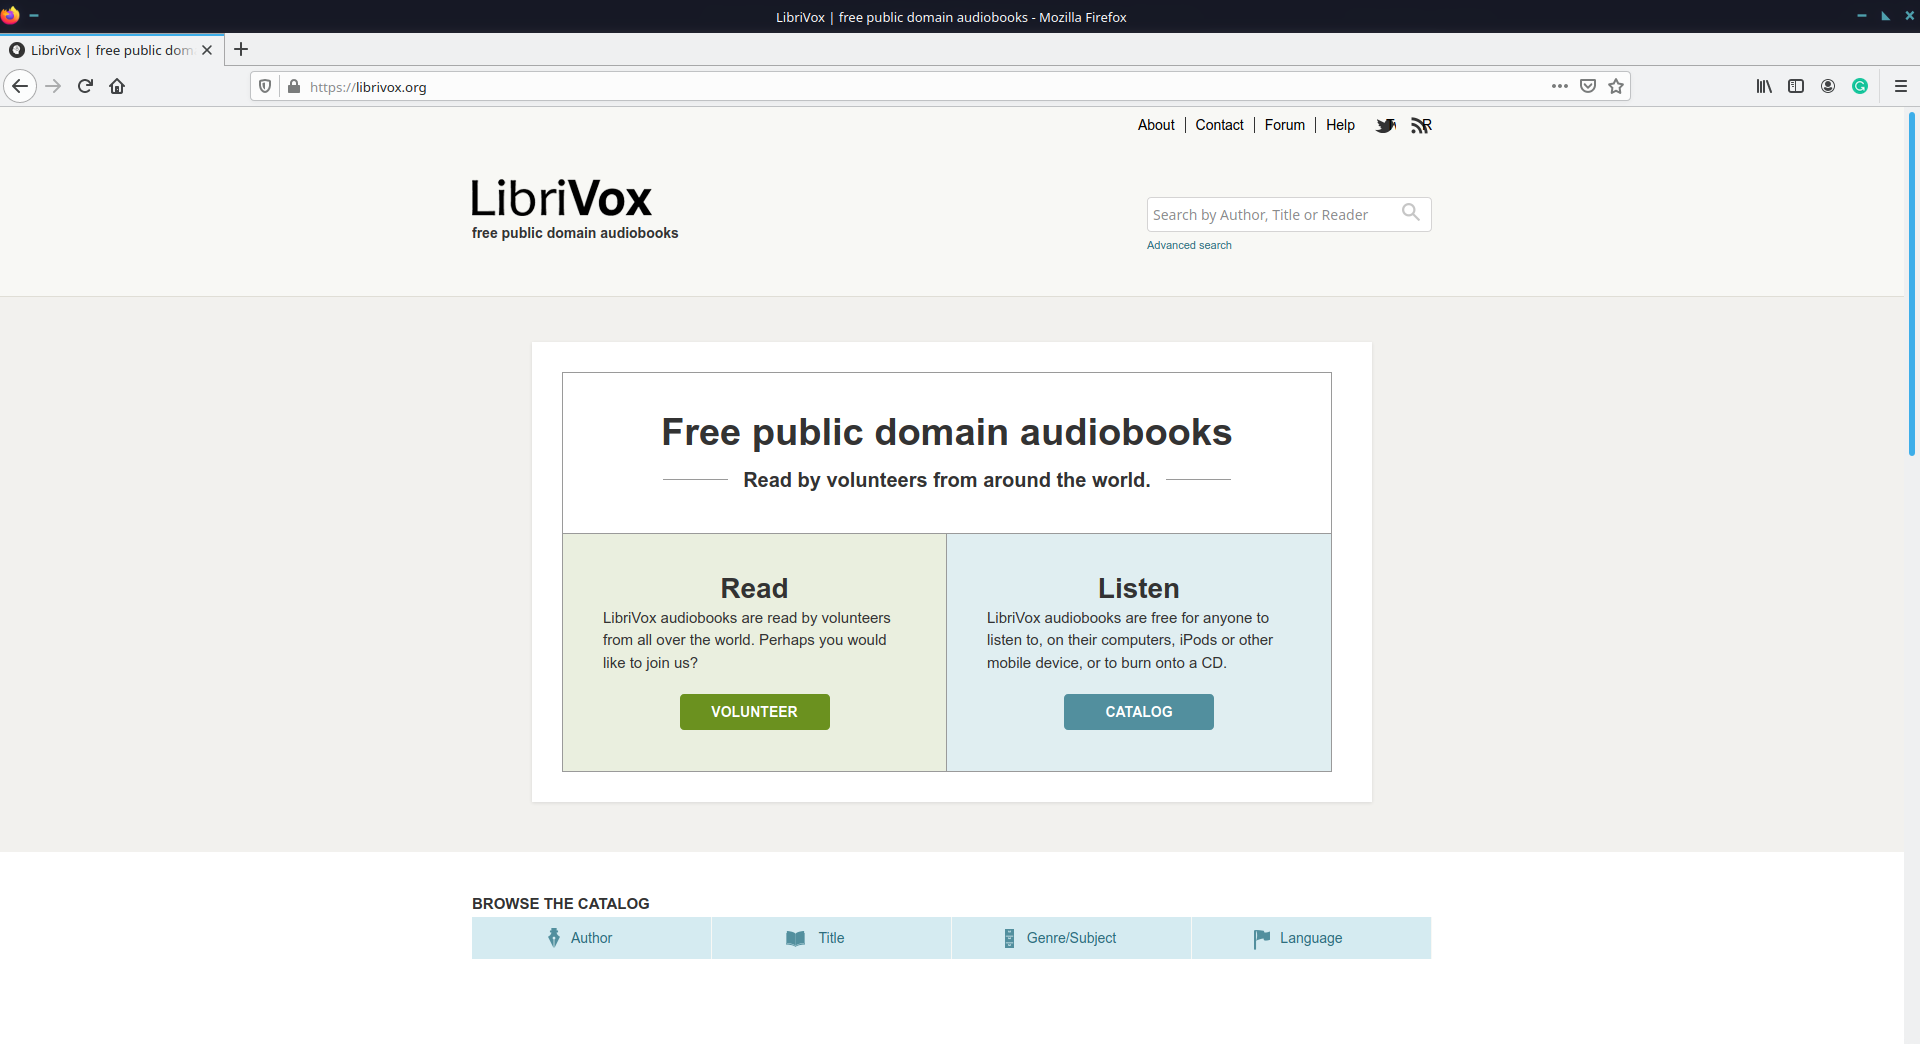
\includegraphics[width=\columnwidth]{figures/LibriVox_cover.png}
	}      
	\caption{LibriVox página principal}
	\label{fig: librivox_cover}
\end{figure}
\subsubsection{Análisis de la \acrshort{URL}}
A continuación se selecciona el filtro del lenguaje puesto que el trabajo se va a entrar para audiolibros en castellano. El navegador se actualiza y muestra el siguiente contenido en la barra de dirección.
\begin{center}
	\fbox{%
	\tiny{https://librivox.org/search?primary\_key=5\&search\_category=language\&search\_page=1\&search\_form=get\_results}
	}%
\end{center}
De esta información se pueden extraer que existen varios tipos de información separados por el caracter \textbf{\&} organizados como \textbf{atributo=valor}. A continuación se analizan cada uno de los filtros:
\begin{itemize}
	\item \textbf{primary\_key} es el valor del campo principal de búsqueda, en este paso como se busca por la categoría \textbf{language} el valor \textbf{5} representa el \textbf{español}.
	\item \textbf{search\_category} esta campo representa la categoría mediante la cual se están haciendo la búsqueda. Otros posibles valores serían \textbf{author}, \textbf{title}, entre otros.
	\item \textbf{search\_page} este campo representa la página actual de búsqueda. Por consiguiente para cambiar de página dentro del mismo idioma se debe ir incrementando este número
\end{itemize}
\subsubsection{Análisis del sitio web con herramientas de desarrollador}
El siguiente paso consiste en analizar cómo están la información en la paǵina web. En este caso, la lista de resultados la devuelve un JavaScript que tarda unos segundos en cargar. Después de la carga se puede empezar a analizar el contenido como muestra la figura \ref{fig: librivox_inspect}
\begin{figure}[ht!]
	\centering
	\resizebox{\textwidth}{!}{
		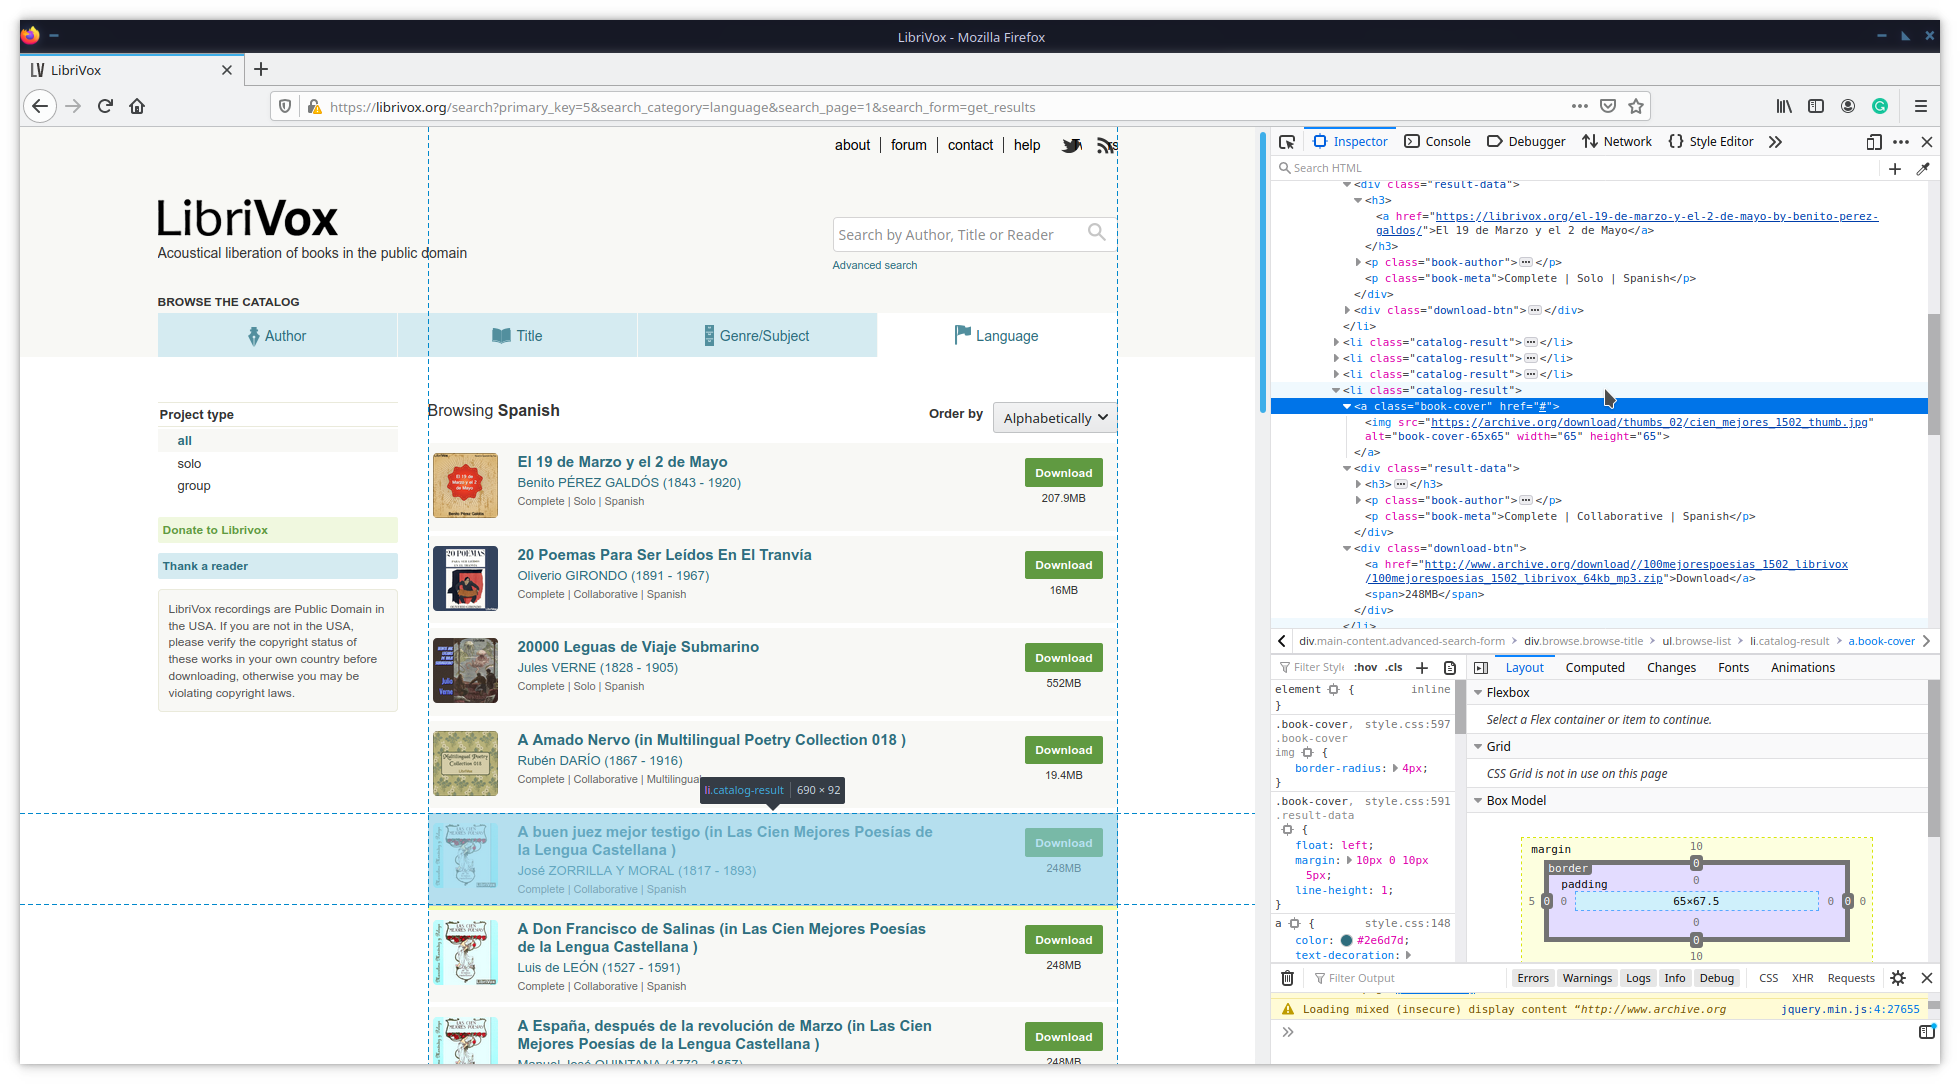
\includegraphics[width=\columnwidth]{figures/LibriVox_inspect.png}
	}      
	\caption{LibriVox analizado con el inspector de Firefox}
	\label{fig: librivox_inspect}
\end{figure}

\begin{lstlisting}[style=HTML,basicstyle=\tiny\ttfamily, caption={Ejemplo de la información contenida para uno de los libros},captionpos=b, label={lst: librivox_book}]
<li class="catalog-result">
  <a href="#" class="book-cover">
    <img src="https://archive.org/download/thumbs_02/cien_mejores_1502_thumb.jpg"
       alt="book-cover-65x65" width="65" height="65">
  </a>
  <div class="result-data">
    <h3>
    <a href="https://librivox.org/las-cien-mejores-poesias-de-la-lengua-castellana-by-marcelino-menendez-y-pelayo/">
      A buen juez mejor testigo (in Las Cien Mejores Poesías de la Lengua Castellana )
    </a></h3>
    <p class="book-author"> <a href="https://librivox.org/author/11155">José ZORRILLA Y MORAL (1817 - 1893)</a> </p>
    <p class="book-meta"> Complete | Collaborative | Spanish</p>
  </div>	
  <div class="download-btn">
    <a href="http://www.archive.org/download//100mejorespoesias_1502_librivox/100mejorespoesias_1502_librivox_64kb_mp3.zip">
      Download
    </a>
    <span>248MB</span>
  </div>
</li>
\end{lstlisting}
Los datos de los libros que devuelve la búsqueda para dicha página se encuentran dentro de los bloques \textcolor{editorBlue}{$<$}\textcolor{editorPink}{li class}\textcolor{editorBlue}{=}\textcolor{editorPurple}{''catalog-result''}\textcolor{editorBlue}{$>$}. El ejemplo del contenido de uno de ellos se encuentra en el listado de código \ref{lst: librivox_book}. Se puede ver que hay mucha información sobre el libro, inclusive, la \gls{URL} de descarga del mismo.
\subsubsection{Extracción y almacenamiento de la información}
Para la extracción de la información se desarrolló un algoritmo basado en un webdriver con la librería \textit{Selenium} y en el parseador de \gls{HTML} \textit{BeautifulSoup}. El algoritmo consiste en ir incrementando el valor de página y buscando toda la información de los libros en dicha página después de que la Query haya cargado. Para esto se busca el valor de la última página; si este valor es nulo, se incrementa un segundo el tiempo aleatorio de espera para el parseo de los datos. Si el valor obtenido es distinto de nulo, significa que la página ha cargado, entonces, se parsea la información de todos los libros en la página y se almacena en una base de datos \textit{SQLite}. En la figura \ref{fig: librivox_scraper_flowchart} se puede ver el diagrama de flujo del código para la parte del scraper y en \ref{lst: librivox_scraper} se puede ver el código que implementa la clase.

\begin{figure}[ht!]
	\centering
	\resizebox{!}{0.8\textheight}{
		\begin{tikzpicture}
		\tikzstyle{box} = [draw,inner sep=7,minimum size=57,line 
		width=1, very thick, draw=black, fill=black!20, text width=120, text centered]
		\tikzstyle{invisible} = [outer sep=0,inner sep=0,minimum size=0]
		\tikzstyle{stealth} = [-stealth]
		
		\tikzstyle{decision} = [diamond, draw, fill=yellow!20, 
		text width=6em, text badly centered, node distance=3cm, inner sep=0pt]
		\tikzstyle{block} = [rectangle, draw, fill=gray!20, 
		text width=12em, text centered, rounded corners, minimum height=4em]
		\tikzstyle{small_block} = [circle, draw, fill=white!20, 
		text width=0em, text centered, rounded corners, minimum height=0em]    
		\tikzstyle{cloud} = [draw, ellipse,fill=red!20, node distance=3cm,
		minimum height=2em]
		
		\node [cloud] (v8) at (0,3.5) {\textbf{Start}};
		\node [block] (v3) at (0,1.5) {\vspace*{-0pt}\begin{itemize}
			\item lastPage=0 \vspace*{-0pt}
			\item increaseSleep=0 \vspace*{-0pt}
			\item page=1 \vspace*{-0pt}
			\item availablePage=True
			\end{itemize}};
		\node [block] (v2) at (0,-1) {Update URL\\ GET URL};
		\node [block] (v4) at (0,-3) {Sleep[random(0.5,1) + increaseSlepp]};
		\node [block] (v5) at (0,-5) {Parse lastPageNode};
		\node [decision] (v6) at (0,-8) {lastPageNode == Null?};
		\node [block] (v1) at (-3.5,-10) {increaseSleep+=1};
		\node [block] (v7) at (3.5,-10) {increaseSleep=0};
		\draw [stealth,out=180,in=180] (v1) edge (v2);
		\draw [stealth] (v3) edge (v2);
		\draw [stealth] (v2) edge (v4);
		\draw [stealth] (v4) edge (v5);
		\draw [stealth] (v5) edge (v6);
		\draw [stealth,out=180,in=90] (v6) edge node[anchor=east]{YES} (v1);
		\draw [stealth,out=0,in=90] (v6) edge node[anchor=west]{NO} (v7);
		\draw [stealth] (v8) edge (v3);
		\node [decision] (v9) at (3.5,-13) {lastPage == 0?};
		\node [block] (v10) at (-1,-14.5) {Update lastPage val(lastPageNode)};
		\draw [stealth,out=180,in=90] (v9) edge node [anchor=south east]{YES} (v10);
		\node [block] (v13) at (3.5,-16.5) {Parse information for every book in the query};
		\node [block] (v12) at (-1,-21) {page+=1};
		\node [decision] (v11) at (3.5,-19.5) {page == lastPage?};
		\draw [stealth,out=180,in=90] (v11) edge  node [anchor=south east]{NO} (v12);
		\draw [stealth,out=180,in=180] (v12) edge (v2);
		\draw [stealth] (v9) edge node [anchor=south east]{NO} (v13);
		\draw [stealth] (v7) edge (v9);
		\draw [stealth] (v13) edge (v11);
		\draw [stealth,out=270,in=180] (v10) edge (v13);
		\node [cloud] (v14) at (5.5,-21) {\textbf{end}};
		\draw [stealth,out=0,in=90] (v11) edge node[anchor=west]{YES} (v14);
		\end{tikzpicture}
	}      
	\caption{Diagrama de flujo para el scraper de LibriVox}
	\label{fig: librivox_scraper_flowchart}
\end{figure}

Una vez que la información de los libros está almacenada en la base de datos, se puede pasar a descargar los libros desde sus correspondientes \glspl{URL}. Para ello se hacen las peticiones \gls{GET} correspondientes para la descarga de los audios. Una vez descargados, se descomprimen y se analizan para extraerles los metadatos que son almacenados en la base de datos. En \ref{lst: audio_manager} se puede ver el código que implementa esta parte del trabajo.

\section{Ruido}
Para el ruido se han seleccionado vídeos de YouTube con ruidos urbanos, murmullo, lluvia y ruido característico de un centro de procesado de datos. Estos vídeos se han descargado mediante la librería \textit{youtube\_dl} y se les ha extraído el sonido así como información referente a la tasa de muestro, duración y el número de canales. Esta información junto con la localización de almacenamiento se ha introducido en la base de datos de SQLite. En \ref{lst: noise_manager} se puede ver el código que implementa esta parte del proyecto.

	\clearpage
	\chapter{Análisis exploratorio de datos}\label{ch: eda}
Para el análisis exploratorio de datos, en primer lugar, se van a analizar la dimensión y las propiedades de datos a través una serie de querys a la base de datos donde se han almacenado los metadatos del dataset.

Los metadatos han sido divididos en dos tablas en función del lugar a dónde pertenecen. La primera tabla hace referencia a las pistas de los audiolibros y la segunda a los ruidos. La tabla \ref{tab: audio_book_table} presenta la columnas que contiene la tabla de las pistas de audio y la \ref{tab: noise_table} los metadatos de las pistas de ruido.

\begin{table} [ht!]
	\centering
	\resizebox{\columnwidth}{!}{%
		\begin{tabular}{L{5cm} C{3cm} L{15cm}}
			\toprule
			\textbf{Nombre} & \textbf{Tipo de dato} & \textbf{Descripción}\\ \midrule
			id & int & Identificador de la pista de audio \\ \midrule
			book\_name\_dummy & text & Nombre del libro con caracteres \acrshort{ASCII} reducidos \\ \midrule
			book\_name & text & Nombre completo del libro \\ \midrule
			book\_author & text & Autor del libro \\ \midrule
			book\_url & text & \gls{URL} de descarga del libro \\ \midrule
			book\_language & text & Lenguaje del libro \\ \midrule
			book\_path & text & Dirección de almacenamiento del libro comprimido \\ \midrule
			book\_n\_tracks & int & Número de pistas del libro \\ \midrule
			track\_name & text & Nombre de la pista de audio \\ \midrule
			track\_path & text & Directorio de almacenamiento de la pista de audio \\ \midrule
			track\_channels & int & Número de canales de la pista de audio \\ \midrule
			track\_sample\_rate & int & Tasa de muestreo de la pista de audio \\ \midrule
			track\_duration & real & Duración de la pista de audio \\ \midrule
			track\_status & text & Estado del archivo (OK\arrowTikz{0}descargado, DELETED\arrowTikz{0}eliminado) \\ \midrule
			track\_insert\_datetime & int & Fecha y hora de inserción del registro \\ \bottomrule
		\end{tabular}
	}
	\vspace*{3pt}
	\caption{Columnas de la tabla pista de los audiolibros}\label{tab: audio_book_table}
\end{table}

\begin{table} [ht!]
	\centering
	\resizebox{\columnwidth}{!}{%
		\begin{tabular}{L{5cm} C{3cm} L{15cm}}
			\toprule
			\textbf{Nombre} & \textbf{Tipo de dato} & \textbf{Descripción}\\ \midrule
			id & int & Identificador de la pista de ruido \\ \midrule
			name & text & Nombre del ruido que coincide con el nombre del archivo \acrshort{ASCII} reducidos \\ \midrule
			url & text & \gls{URL} de descarga del video que contiene el ruido \\ \midrule
			path & text & Dirección de almacenamiento de la pista de ruido \\ \midrule
			channels & int & Número de canales de la pista de ruido \\ \midrule
			sample\_rate & int & Tasa de muestreo de la pista de ruido \\ \midrule
			duration & real & Duración de la pista de ruido \\ \midrule
			status & text & Estado del archivo (OK\arrowTikz{0}descargado, DELETED\arrowTikz{0}eliminado) \\ \midrule
			insert\_datetime & int & Fecha y hora de inserción del registro \\ \bottomrule
		\end{tabular}
	}
	\vspace*{3pt}
	\caption{Columnas de la tabla con los metadatos de las pista de ruido}\label{tab: noise_table}
\end{table}

A partir de las tablas se pueden sacar datos que den una idea de la dimensión del problema y si los datos son compatibles entre ellos o no. Dos pistas de audio pueden ser no compatibles porque el algoritmo se diseña para una tasa de muestreo estática y, las pistas de audio o ruido, no tienen por qué tener tasas de muestreo que sean múltiplos y divisores comunes de la del modelo. En primer lugar se pueden ver la duración total de las pista de audiolibros y de ruido, para ello simplemente se lanza una query \textbf{agregando por el campo duración} con la función \textbf{SUM} como muestra la tabla \ref{tab: duration}.
\begin{table} [h!]
	\centering
	\resizebox{!}{!}{%
		\begin{tabular}{L{3cm} C{3cm} C{3cm}}
			\toprule
			\textbf{Tipo de pista} & \textbf{Duración [horas]} & \textbf{Tasas de muestreo [$\frac{muestras}{segundo}$]}\\ \midrule
			Audiolibros & 707.70 & [22050]\\ \midrule
			Ruido & 52.91 & [44100, 48000]\\ \bottomrule
		\end{tabular}
	}
	\vspace*{3pt}
	\caption{Duración total de todas las pistas}\label{tab: duration}
\end{table}

Otra métrica interesante es, como se comentó anteriormente, la compatibilidad de tasas de muestreo. Para ello se \textbf{agrega por el campo tasa de muestreo} con la función \textbf{DISTINCT}. El resultado se encuentra en la tabla \ref{tab: duration}.

A parte de obtener métricas, se pueden analizar la consistencia de los datos. Por ejemplo, se podría analizar si existen algunas pista de audio que se encuentren en varios libros. Esto se daría si la plataforma de almacenamiento metiera varios libros en una misma \gls{URL} de descarga. En \ref{lst: repeat_track} se puede ver el código que implementa la query. El resultado de esta query es que hay \textbf{162} registros que se encuentran, como mínimo, dos veces.

\begin{lstlisting}[style=SQL,basicstyle=\tiny\ttfamily, caption={Query para obtener las pistas repetidas en varios libros},captionpos=b, label={lst: repeat_track}]
SELECT track_name, COUNT(*) AS c
FROM audio_books_tracks
GROUP BY track_name
HAVING c > 1
ORDER BY c DESC
\end{lstlisting}

Como la query da resultados distintos de \textbf{NULL}, hay pistas de audiolibros que se han contado varias veces falseando las estadísticas. Realizando una query con alguno de los resultados se confirma que existen pistas que se encuentran en varios libros y, por tanto, son registros repetidos. En la tabla \ref{tab: repeat_registers} se puede ver una de las pistas que se encuentra repetida. Con este tipo de queries se puede ver que de los \textbf{4227} registros, únicos son \textbf{2802}.
\begin{table} [h!]
	\centering
	\resizebox{\textwidth}{!}{%
		\begin{tabular}{L{0.6cm} L{7cm} L{10cm}}
			\toprule
			\textbf{id} & \textbf{book\_name} & \textbf{track\_name}\\ \midrule
			1351 & Antología de Cuentos Fantásticos & antologiacuentosfantasticos\_01\_various\_64kb.mp3 \\ \midrule
			3410 & Coppelius (1ra Parte) (in  Antología de Cuentos Fantásticos ) & antologiacuentosfantasticos\_01\_various\_64kb.mp3 \\ \midrule
			3935 & De lo que aconteció a un deán de Santiago con don Illan el mágico, que moraba en Toledo (in  Antología de Cuentos Fantásticos ) & antologiacuentosfantasticos\_01\_various\_64kb.mp3 \\ \midrule
		\end{tabular}
	}
	\vspace*{3pt}
	\caption{Ejemplo de registros repetidos}\label{tab: repeat_registers}
\end{table}





	\clearpage
	\chapter{Diseño e implementación de los modelos o técnicas necesarias}\label{ch: modelDesign}
En el capítulo \ref{ch: eda} se expuso la naturaleza espectral del problema, sería lógico pensar que una forma de reducir el ruido de una conversación sería filtrar para todas aquellas frecuencias que no sean la frecuencia fundamental y sus armónicos característicos del habla de una persona. Esta solución sería perfectamente válida y se ajusta a la necesidad del problema pero tiene un gran inconveniente, el tuneo fino y adaptable de los filtros.

Para poder filtrar las frecuencias fundamentales, éstas deben ser encontradas y esa no es tarea fácil. Además dichas frecuencias varían en el tiempo de modo que los filtros deben adaptarse a cada instante a la nuevas frecuencias, esto complica la tarea aún más. Existe una familia de filtros llamados \textit{comb}, peine, que consisten en una serie de picos equi-espaciados creando mediante retardos de la propia señal perfectamente válidos para la detección y filtrado de la frecuencia fundamental\cite{1035730}, de nuevo el tuneo fino es una tarea compleja. Por ello, este trabajo propone un sistema completo de redes neuronales en el cual no se aplican técnicas de clásicas de \gls{DSP}.

Dado que el en capítulo \ref{ch: eda} se presentaron los análisis en frecuencia y en tiempo, quedó de manifiesto que en el dominio de la frecuencia las pistas con ruido y sin él se diferencian mucho. Por esta razón el algoritmo que se propone en este trabajo se basa en el análisis de audio en el dominio de la frecuencia, para ello se deben pre-procesar los datos eligiendo unos parámetros que determinarán como serán los datos, a continuación se explican los algoritmos matemáticos de las transformaciones que se van a aplicar a las pistas de audio.

\section{Preprocesado de datos de audio para el modelo}
Los modelos se van a alimentar de \glspl{FFT} calculadas a partir de las muestras temporales de los audios. Estas \glspl{FFT} deben ser lo suficientemente precisas para poder reconstruir el audio pero sin usar una gran cantidad de muestras para no producir un retraso en la señal.

Se ha realizado una prueba experimental para calcular a que tasa de muestreo el audio sigue siendo posible reconstruir. A menor tasa de muestreo, para la misma resolución en frecuencia, la \gls{FFT} resultante tiene menos puntos, i.e., menor carga computacional. Es importante este ajuste porque reducir la tasa de muestreo a la mitad o un cuarto implica reducir el vector de entrada de la red a la mitad o un cuarto, respectivamente. Adicionalmente sólo son procesados la mitad de los datos de la salida de la transformada de Fourier. Esto es debido a que la respuesta de una transformada es un vector de números complejos y de éstos sólo se procesa el módulo. La fase se deja intacta y se usa para reconstruir el vector complejo junto con el módulo que sale del modelo. La figura \ref{fig: model_schema} presenta un esquema de cuáles son las entradas y salidas del modelo.

\begin{figure}[ht!]
	\centering
	\resizebox{\textwidth}{!}{
		\begin{tikzpicture}
		\tikzstyle{box} = [draw,inner sep=7,minimum size=57,line 
		width=1, very thick, draw=black, fill=black!20, text width=100, text centered]
		\tikzstyle{invisible} = [outer sep=0,inner sep=0,minimum size=0]
		\tikzstyle{stealth} = [-stealth, very thick]
		\begin{scope}[shift={(0.5,0)}]		
		\begin{scope}[shift={(-3.5,3.1)}, scale=0.5]
		\node [invisible] at (-1.2,1.7) {$FFT_n$};
		\draw (-3,0.5) node [invisible] {} -- (-2.8,0.3) node [invisible] {} -- (-2.6,0.2) node [invisible] {} -- (-2.4,0.8) node [invisible] {} -- (-2.2,0.2) node [invisible] {} -- (-2,0.3) node [invisible] {} -- (-1.9,0.2) node [invisible] {} -- (-1.8,0.4) node [invisible] {} -- (-1.7,0.2) node [invisible] {} -- (-1.6,1.4) node [invisible] {} -- (-1.5,0.2) node [invisible] {} -- (-1.3,0.3) node [invisible] (v4) {};
		\node [invisible] (v2) at (-3,1.6) {};
		\node [invisible] (v1) at (-3,-0.4) {};
		\node [invisible] (v3) at (0.6,-0.4) {};
		\draw [stealth] (v1) edge (v2);
		\draw [stealth] (v1) edge (v3);
		\draw [stealth](v4);
		\draw (v4) -- (-1.2,0.2) node [invisible] {} -- (-1.1,0.4) node [invisible] {} -- (-1,0.2) node [invisible] {} -- (-0.8,0.8) node [invisible] {} -- (-0.7,0.2) node [invisible] {} -- (-0.5,0.3) node [invisible] {} -- (-0.4,0.2) node [invisible] {} -- (-0.2,0.3) node [invisible] {} -- (-0.1,0.2) node [invisible] {} -- (0.1,1.1) node [invisible] {} -- (0.3,0.2) node [invisible] {};
		\end{scope}
		\begin{scope}[shift={(-3.1,1.8)}, scale=0.5]
		\node [invisible] at (-1.2,1.7) {$FFT_{n-1}$};
		\draw (-3,0.5) node [invisible] {} -- (-2.8,0.3) node [invisible] {} -- (-2.6,0.2) node [invisible] {} -- (-2.4,0.8) node [invisible] {} -- (-2.2,0.2) node [invisible] {} -- (-2,0.3) node [invisible] {} -- (-1.9,0.2) node [invisible] {} -- (-1.8,0.4) node [invisible] {} -- (-1.7,0.2) node [invisible] {} -- (-1.6,1.4) node [invisible] {} -- (-1.5,0.2) node [invisible] {} -- (-1.3,0.3) node [invisible] (v4) {};
		\node [invisible] (v2) at (-3,1.6) {};
		\node [invisible] (v1) at (-3,-0.4) {};
		\node [invisible] (v3) at (0.6,-0.4) {};
		\draw [stealth] (v1) edge (v2);
		\draw [stealth] (v1) edge (v3);
		\draw [stealth](v4);
		\draw (v4) -- (-1.2,0.2) node [invisible] {} -- (-1.1,0.4) node [invisible] {} -- (-1,0.2) node [invisible] {} -- (-0.8,0.8) node [invisible] {} -- (-0.7,0.2) node [invisible] {} -- (-0.5,0.3) node [invisible] {} -- (-0.4,0.2) node [invisible] {} -- (-0.2,0.3) node [invisible] {} -- (-0.1,0.2) node [invisible] {} -- (0.1,1.1) node [invisible] {} -- (0.3,0.2) node [invisible] {};
		\end{scope}
		\begin{scope}[shift={(-1.5,-0.9)}, scale=0.5]
		\node [invisible] at (-1.2,1.7) {$FFT_2$};
		\draw (-3,0.5) node [invisible] {} -- (-2.8,0.3) node [invisible] {} -- (-2.6,0.2) node [invisible] {} -- (-2.4,0.8) node [invisible] {} -- (-2.2,0.2) node [invisible] {} -- (-2,0.3) node [invisible] {} -- (-1.9,0.2) node [invisible] {} -- (-1.8,0.4) node [invisible] {} -- (-1.7,0.2) node [invisible] {} -- (-1.6,1.4) node [invisible] {} -- (-1.5,0.2) node [invisible] {} -- (-1.3,0.3) node [invisible] (v4) {};
		\node [invisible] (v2) at (-3,1.6) {};
		\node [invisible] (v1) at (-3,-0.4) {};
		\node [invisible] (v3) at (0.6,-0.4) {};
		\draw [stealth] (v1) edge (v2);
		\draw [stealth] (v1) edge (v3);
		\draw [stealth](v4);
		\draw (v4) -- (-1.2,0.2) node [invisible] {} -- (-1.1,0.4) node [invisible] {} -- (-1,0.2) node [invisible] {} -- (-0.8,0.8) node [invisible] {} -- (-0.7,0.2) node [invisible] {} -- (-0.5,0.3) node [invisible] {} -- (-0.4,0.2) node [invisible] {} -- (-0.2,0.3) node [invisible] {} -- (-0.1,0.2) node [invisible] {} -- (0.1,1.1) node [invisible] {} -- (0.3,0.2) node [invisible] {};
		\end{scope}
		\begin{scope}[shift={(-1.1,-2.2)}, scale=0.5]
		\node [invisible] at (-1.2,1.7) {$FFT_1$};
		\draw (-3,0.5) node [invisible] {} -- (-2.8,0.3) node [invisible] {} -- (-2.6,0.2) node [invisible] {} -- (-2.4,0.8) node [invisible] {} -- (-2.2,0.2) node [invisible] {} -- (-2,0.3) node [invisible] {} -- (-1.9,0.2) node [invisible] {} -- (-1.8,0.4) node [invisible] {} -- (-1.7,0.2) node [invisible] {} -- (-1.6,1.4) node [invisible] {} -- (-1.5,0.2) node [invisible] {} -- (-1.3,0.3) node [invisible] (v4) {};
		\node [invisible] (v2) at (-3,1.6) {};
		\node [invisible] (v1) at (-3,-0.4) {};
		\node [invisible] (v3) at (0.6,-0.4) {};
		\draw [stealth] (v1) edge (v2);
		\draw [stealth] (v1) edge (v3);
		\draw [stealth](v4);
		\draw (v4) -- (-1.2,0.2) node [invisible] {} -- (-1.1,0.4) node [invisible] {} -- (-1,0.2) node [invisible] {} -- (-0.8,0.8) node [invisible] {} -- (-0.7,0.2) node [invisible] {} -- (-0.5,0.3) node [invisible] {} -- (-0.4,0.2) node [invisible] {} -- (-0.2,0.3) node [invisible] {} -- (-0.1,0.2) node [invisible] {} -- (0.1,1.1) node [invisible] {} -- (0.3,0.2) node [invisible] {};
		\end{scope}
		\node [circle, fill] at (-3.6,1.2) {};
		\node [circle, fill] at (-3.2,0.8) {};
		\node [circle, fill] at (-2.8,0.4) {};
		\draw [dashed, thick] (-5.5,6) node [invisible] (v5) {} -- (-5.5,-3.5) -- (-0.5,-3.5) -- (-0.5,6) -- (v5);
		\node [invisible] (v6) at (-0.5,0.75) {};
		\end{scope}
		
		\begin{scope}[shift={(10.5,0)}]		
		\begin{scope}[shift={(-1.2,3.1)}, scale=0.5]
		\node [invisible] at (-1.2,1.7) {$FFT_n$};
		\draw (-3,0.5) node [invisible] {} -- (-2.8,0.3) node [invisible] {} -- (-2.6,0.2) node [invisible] {} -- (-2.4,0.8) node [invisible] {} -- (-2.2,0.2) node [invisible] {} -- (-2,0.3) node [invisible] {} -- (-1.9,0.2) node [invisible] {} -- (-1.8,0.4) node [invisible] {} -- (-1.7,0.2) node [invisible] {} -- (-1.6,1.4) node [invisible] {} -- (-1.5,0.2) node [invisible] {} -- (-1.3,0.3) node [invisible] (v4) {};
		\node [invisible] (v2) at (-3,1.6) {};
		\node [invisible] (v1) at (-3,-0.4) {};
		\node [invisible] (v3) at (0.6,-0.4) {};
		\draw [stealth] (v1) edge (v2);
		\draw [stealth] (v1) edge (v3);
		\draw [stealth](v4);
		\draw (v4) -- (-1.2,0.2) node [invisible] {} -- (-1.1,0.4) node [invisible] {} -- (-1,0.2) node [invisible] {} -- (-0.8,0.8) node [invisible] {} -- (-0.7,0.2) node [invisible] {} -- (-0.5,0.3) node [invisible] {} -- (-0.4,0.2) node [invisible] {} -- (-0.2,0.3) node [invisible] {} -- (-0.1,0.2) node [invisible] {} -- (0.1,1.1) node [invisible] {} -- (0.3,0.2) node [invisible] {};
		\end{scope}
		\begin{scope}[shift={(-1.7,1.8)}, scale=0.5]
		\node [invisible] at (-1.2,1.7) {$FFT_{n-1}$};
		\draw (-3,0.5) node [invisible] {} -- (-2.8,0.3) node [invisible] {} -- (-2.6,0.2) node [invisible] {} -- (-2.4,0.8) node [invisible] {} -- (-2.2,0.2) node [invisible] {} -- (-2,0.3) node [invisible] {} -- (-1.9,0.2) node [invisible] {} -- (-1.8,0.4) node [invisible] {} -- (-1.7,0.2) node [invisible] {} -- (-1.6,1.4) node [invisible] {} -- (-1.5,0.2) node [invisible] {} -- (-1.3,0.3) node [invisible] (v4) {};
		\node [invisible] (v2) at (-3,1.6) {};
		\node [invisible] (v1) at (-3,-0.4) {};
		\node [invisible] (v3) at (0.6,-0.4) {};
		\draw [stealth] (v1) edge (v2);
		\draw [stealth] (v1) edge (v3);
		\draw [stealth](v4);
		\draw (v4) -- (-1.2,0.2) node [invisible] {} -- (-1.1,0.4) node [invisible] {} -- (-1,0.2) node [invisible] {} -- (-0.8,0.8) node [invisible] {} -- (-0.7,0.2) node [invisible] {} -- (-0.5,0.3) node [invisible] {} -- (-0.4,0.2) node [invisible] {} -- (-0.2,0.3) node [invisible] {} -- (-0.1,0.2) node [invisible] {} -- (0.1,1.1) node [invisible] {} -- (0.3,0.2) node [invisible] {};
		\end{scope}
		\begin{scope}[shift={(-3.2,-0.9)}, scale=0.5]
		\node [invisible] at (-1.2,1.7) {$FFT_2$};
		\draw (-3,0.5) node [invisible] {} -- (-2.8,0.3) node [invisible] {} -- (-2.6,0.2) node [invisible] {} -- (-2.4,0.8) node [invisible] {} -- (-2.2,0.2) node [invisible] {} -- (-2,0.3) node [invisible] {} -- (-1.9,0.2) node [invisible] {} -- (-1.8,0.4) node [invisible] {} -- (-1.7,0.2) node [invisible] {} -- (-1.6,1.4) node [invisible] {} -- (-1.5,0.2) node [invisible] {} -- (-1.3,0.3) node [invisible] (v4) {};
		\node [invisible] (v2) at (-3,1.6) {};
		\node [invisible] (v1) at (-3,-0.4) {};
		\node [invisible] (v3) at (0.6,-0.4) {};
		\draw [stealth] (v1) edge (v2);
		\draw [stealth] (v1) edge (v3);
		\draw [stealth](v4);
		\draw (v4) -- (-1.2,0.2) node [invisible] {} -- (-1.1,0.4) node [invisible] {} -- (-1,0.2) node [invisible] {} -- (-0.8,0.8) node [invisible] {} -- (-0.7,0.2) node [invisible] {} -- (-0.5,0.3) node [invisible] {} -- (-0.4,0.2) node [invisible] {} -- (-0.2,0.3) node [invisible] {} -- (-0.1,0.2) node [invisible] {} -- (0.1,1.1) node [invisible] {} -- (0.3,0.2) node [invisible] {};
		\end{scope}
		\begin{scope}[shift={(-3.7,-2.2)}, scale=0.5]
		\node [invisible] at (-1.2,1.7) {$FFT_1$};
		\draw (-3,0.5) node [invisible] {} -- (-2.8,0.3) node [invisible] {} -- (-2.6,0.2) node [invisible] {} -- (-2.4,0.8) node [invisible] {} -- (-2.2,0.2) node [invisible] {} -- (-2,0.3) node [invisible] {} -- (-1.9,0.2) node [invisible] {} -- (-1.8,0.4) node [invisible] {} -- (-1.7,0.2) node [invisible] {} -- (-1.6,1.4) node [invisible] {} -- (-1.5,0.2) node [invisible] {} -- (-1.3,0.3) node [invisible] (v4) {};
		\node [invisible] (v2) at (-3,1.6) {};
		\node [invisible] (v1) at (-3,-0.4) {};
		\node [invisible] (v3) at (0.6,-0.4) {};
		\draw [stealth] (v1) edge (v2);
		\draw [stealth] (v1) edge (v3);
		\draw [stealth](v4);
		\draw (v4) -- (-1.2,0.2) node [invisible] {} -- (-1.1,0.4) node [invisible] {} -- (-1,0.2) node [invisible] {} -- (-0.8,0.8) node [invisible] {} -- (-0.7,0.2) node [invisible] {} -- (-0.5,0.3) node [invisible] {} -- (-0.4,0.2) node [invisible] {} -- (-0.2,0.3) node [invisible] {} -- (-0.1,0.2) node [invisible] {} -- (0.1,1.1) node [invisible] {} -- (0.3,0.2) node [invisible] {};
		\end{scope}
		\node [circle, fill] at (-2.8,1.2) {};
		\node [circle, fill] at (-3.2,0.8) {};
		\node [circle, fill] at (-3.6,0.4) {};
		\draw [dashed, thick] (-5.5,6) node [invisible] (v5) {} -- (-5.5,-3.5) -- (-0.5,-3.5) -- (-0.5,6) -- (v5);
		\node [invisible] (v8) at (-5.5,0.75) {};
		\end{scope}
		
		\node [box,text width=60] (v7) at (2.5,0.75) {Modelo};
		
		
		\node [invisible] at (-2.5,5.5) {Módulo de FFT con ruido};
		\node [invisible] at (7.5,5.5) {Módulo de FFT sin ruido};
		\draw [stealth] (v6) edge (v7);
		\draw [stealth] (v7) edge (v8);
		\node [box] (v9) at (-8.5,7) {$Tiempo\xrightarrow{FFT}Frecuencia$};
		\node [box] (v10) at (13.5,7) {$Frecuencia\xrightarrow{iFFT}Tiempo$};
		\node [invisible] (v11) at (-5,0.75) {};
		\node [invisible] (v12) at (10,0.75) {};
		\draw [stealth,out=0,in=180] (v9) edge node[anchor=south]{Fase} (v10);
		\draw [stealth,out=0,in=180] (v9) edge node[anchor=east]{Módulo}(v11);
		\draw [stealth,out=0,in=180] (v12) edge node[anchor=west]{Módulo}(v10);
		\end{tikzpicture}
	}      
	\caption{Esquema de las entradas y salidas de datos del modelo}
	\label{fig: model_schema}
\end{figure}


\subsection{Generación de datos de entrenamiento y validación}

\section{Modelo de capas \acrshort{LSTM}}

\subsection{Tipos de arquitectura}


	\clearpage
	\chapter{Análisis de los resultados obtenidos}\ref{ch: results}
Este documento es una plantilla realizada en \LaTeX para el \gls{TFM} de la \gls{UEMC}. Este es un ejemplo de bibliografía\cite{Finazzi}.

A continuación un ejemplo de enumeración:
\begin{itemize}
	\item Item 1
	\item Item 2
	\begin{enumerate}
		\item Enum 1
		\item Enum 2
		\item Enum 3
	\end{enumerate}
	\item Item 3
\end{itemize}

Ejemplos de estilo \textbf{negrita}, \textit{cursiva}, \underline{subrayado}, \textbf{\textit{\underline{pack completo}}}. Ecuación en línea $L=\frac{1}{2}\rho V^2 A_{alar}C_l$. La ecuación \ref{eq: massDif} presenta una ecuación alineada.

\begin{align}
	\nonumber
	dm &= \rho dV \\ \nonumber
	&= \rho v dt\cdot dS\cdot \cos{\theta}\\ \nonumber
	&= \rho dt \overrightarrow{v}\cdot d\overrightarrow{S}
\end{align}\label{eq: massDif}
\equationset{Ecuación de la variación de la masa}

\begin{figure}[ht!]
	\centering
	
\includegraphics[width=\columnwidth]{Logo/uemc_logo.pdf}
	\caption{Logo de la \gls{UEMC}}
	\label{fig: UEMC_logo}
\end{figure}
La figura \ref{fig: UEMC_logo} muestra un ejemplo de figura flotante de \LaTeX en el cual se sitúa la imagen en el margen superior de la página. El posicionamiento de los flotantes en \LaTeX lo decide el propio lenguage aunque haya modificadores para "sugerirle" dónde los queremos, el comando \verb_<\FloatBarrier>_ intenta forzar el posicionamiento, aunque no siempre me ha funcionado.

Otro elemento fundamental son las tablas. Existen mil tipos de generación de tablas en \LaTeX; la tabla \ref{tab: bostonHousing} muestra un ejemplo.

\begin{table} [ht!]
	\centering
	\resizebox{0.8\columnwidth}{!}{%
		\begin{tabular}{L{2.5cm} L{15cm}}
			\toprule
			\textbf{Label} & \textbf{Description}\\ \midrule
			\textbf{CRIM} & Per capita crime rate by town \\ \midrule
			\textbf{ZN} & Proportion of residential land zoned for lots over 25000 sq. ft \\ \midrule
			\textbf{INDUS} & Proportion of non-retail business acres per town \\ \midrule
			\textbf{CHAS} & Charles River dummy variable (= 1 if tract bounds river; 0 otherwise) \\ \midrule
			\textbf{NOX} & Nitric oxide concentration (parts per 10 million) \\ \midrule
			\textbf{RM} & Average number of rooms per dwelling \\ \midrule
			\textbf{AGE} & Proportion of owner-occupied units built prior to 1940 \\ \midrule
			\textbf{DIS} & Weighted distances to five Boston employment centers \\ \midrule
			\textbf{RAD} & Index of accessibility to radial highways \\ \midrule
			\textbf{TAX} & Full-value property tax rate per \$10,000 \\ \midrule
			\textbf{PTRATIO} & Pupil-teacher ratio by town \\ \midrule
			\textbf{B} & $1000\left( Bk \text{-} 0.63\right)^2$, where Bk is the proportion of [people of African American descent] by town \\ \midrule
			\textbf{LSTAT} & Percentage of lower status of the population \\ \midrule
			\textbf{MEDV} & Median value of owner-occupied homes in \$1000s \\ \bottomrule
		\end{tabular}
	}
	\vspace*{3pt}
	\caption{Columnas del dataset Boston Housing Price}\label{tab: bostonHousing}
\end{table}

Ejemplo de elevado en texto. Matlab\superscript{\textregistered} es un lenguaje de programación que pertenece a MathWorks\superscript{\texttrademark}. Otro comando útil es generación de flechas embedidas en texto, \arrowTikz{0}~\arrowTikz{45}~\arrowTikz{90}.

\textcolor{red}{Para que este proyecto funcione se debe compilar en \XeLaTeX debido a que utiliza fuentes del sistema operativo tipo \gls{TTF} y/o \gls{OTF}}

\section{Primera sección}
\subsection{Subsección}
\subsubsection{Subsección}

\section*{Sección no numerada}
\section{Segunda sección numerada}
	\clearpage
	\chapter{Conclusiones y planes de mejora}
\lipsum[3-6]
	\appendix
	\chapter{Código de la actividad}

\lstinputlisting[style=Python,basicstyle=\tiny\ttfamily,caption={Código de LibrivoxScraper},captionpos=b, label={lst: librivox_scraper}]{listings/LibrivoxScraper.py}

\lstinputlisting[style=Python,basicstyle=\tiny\ttfamily,caption={Código de gestor de ruido},captionpos=b, label={lst: noise_manager}]{listings/NoiseManager.py}

	\clearpage
	\printglossaries
	\renewcommand{\url}[1]{\href{#1}{link}}
	% Uncomment the following line to print the entire bibliography
	%\nocite{*}
	\bibliographystyle{apacite}
	\bibliography{Bibliography/TFMbibliografia}
	%
\end{document}
%%%%%%%%%%%%%%%%%%%%%%%%%%%%%%%%%%%%%%
